\documentclass[12pt,reqno]{amsart}
\usepackage[pdfborder={0 0 0.5 [3 2]}, plainpages=false]{hyperref}%
\usepackage[left=1in,right=1in,top=1in,bottom=1in]{geometry}%
\usepackage{amsrefs}%
\usepackage{amsmath}
\usepackage{enumerate}
\usepackage{amssymb}                
\usepackage{amsfonts}
\usepackage{amsthm}
\usepackage{bbm}
\usepackage[table,xcdraw]{xcolor}
\usepackage{float}
\usepackage{mathtools}
\usepackage{cool}
\usepackage{graphicx,epsfig}

\usepackage[capitalize,nameinlink]{cleveref}
% Per SIAM Style Manual, "section" should be lowercase
\crefname{section}{section}{sections}
\crefname{subsection}{subsection}{subsections}
\Crefname{section}{Section}{Sections}
\Crefname{subsection}{Subsection}{Subsections}

% Per SIAM Style Manual, "Figure" should be spelled out in references
\Crefname{figure}{Figure}{Figures}

% Per SIAM Style Manual, don't say equation in front on an equation.
\crefformat{equation}{\textup{#2(#1)#3}}
\crefrangeformat{equation}{\textup{#3(#1)#4--#5(#2)#6}}
\crefmultiformat{equation}{\textup{#2(#1)#3}}{ and \textup{#2(#1)#3}}
{, \textup{#2(#1)#3}}{, and \textup{#2(#1)#3}}
\crefrangemultiformat{equation}{\textup{#3(#1)#4--#5(#2)#6}}%
{ and \textup{#3(#1)#4--#5(#2)#6}}{, \textup{#3(#1)#4--#5(#2)#6}}{, and \textup{#3(#1)#4--#5(#2)#6}}

% But spell it out at the beginning of a sentence.
\Crefformat{equation}{#2Equation~\textup{(#1)}#3}
\Crefrangeformat{equation}{Equations~\textup{#3(#1)#4--#5(#2)#6}}
\Crefmultiformat{equation}{Equations~\textup{#2(#1)#3}}{ and \textup{#2(#1)#3}}
{, \textup{#2(#1)#3}}{, and \textup{#2(#1)#3}}
\Crefrangemultiformat{equation}{Equations~\textup{#3(#1)#4--#5(#2)#6}}%
{ and \textup{#3(#1)#4--#5(#2)#6}}{, \textup{#3(#1)#4--#5(#2)#6}}{, and \textup{#3(#1)#4--#5(#2)#6}}

% Make number non-italic in any environment.
\crefdefaultlabelformat{#2\textup{#1}#3}

\def\noi{\noindent}
\def\T{{\mathbb T}}
\def\R{{\mathbb R}}
\def\N{{\mathbb N}}
\def\C{{\mathbb C}}
\def\Z{{\mathbb Z}}
\def\P{{\mathbb P}}
\def\E{{\mathbb E}}
\def\Q{\mathbb{Q}}
\def\ind{{\mathbb I}}

\DeclareMathOperator{\spn}{span}
\DeclareMathOperator{\ran}{range}

\graphicspath{ {images/} }

\newtheorem{lemma}{Lemma}
\newtheorem{theorem}{Theorem}
\newtheorem{corollary}{Corollary}
\newtheorem{definition}{Definition}
\newtheorem{proposition}{Proposition}
\newtheorem{hypothesis}{Hypothesis}
\newtheorem{remark}{Remark}

\begin{document}

\title{Multi-kinks in the discrete Klein-Gordon Equation}

\maketitle

\section{Introduction}

The discrete Klein-Gordon equation (DKG)
\begin{equation}\label{eq:KG}
\ddot{u}_n = d (\Delta_2 u)_n - f(u_n)
\end{equation}
describes the dynamics of an infinitely long, one-dimensional lattice of particles which are harmonically coupled to their neighbors through the discrete second difference operator $\Delta_2$, where $(\Delta_2 u)_n = u_{n+1} - 2 u_n + u_{n-1}$, and are subject to an external, nonlinear, on-site potential $f(u) = V'(u)$ \cite{Karachalios}. The quantity $u_n$ represents the displacement of the particle at site $n$ in the lattice, and the dot represents the derivative with respect to $t$. 

One example of interest is the discrete sine-Gordon equation
\begin{equation}\label{eq:dSG}
	\ddot{u}_n = d (\Delta_2 u)_n - \sin(u_n),
\end{equation}
in which the external potential is periodic. This equation is also known as the Frenkel-Kontorova model, and was introduced in 1938 to describe the dynamics of a crystal lattice near a dislocation core \cite{braun1998}. This equation has since been used in numerous applications, including a mechanical model for a chain of pendulums coupled with elastic springs \cite{Scott1969}, arrays of Josephson junctions \cites{Ustinov1992,Floria1998}, and DNA dynamics \cites{Yomosa1983,Yakushevich1998}. (See \cite{braun2004}*{Chapter 2} for more physical applications of this model.) Another example of interest is the discrete $\phi^4$ variant
\begin{equation}\label{eq:dphi4}
	\ddot{u}_n = d (\Delta_2 u)_n + 2 u_n(1 - u_n^2),
\end{equation}
which has a double well external potential, and has applications to conducting polymers \cite{heeger1988}.

\section{Mathematical background}

The discrete Klein-Gordon equation (DKG) is given by
\begin{equation}\label{eq:KG}
\ddot{u}_n = d (\Delta_2 u)_n - f(u_n),
\end{equation}
where the dot represents the derivative with respect to $t$, $\Delta_2$ is the discrete second difference operator, and $f(u) = V'(u)$ for a smooth potential function $V(u)$. Important versions include the discrete sine-Gordon equation, where $f(u) = -\sin(u)$, and $\phi^4$ variant, where $f(u) = -u(1-u^2)$. The nonlinearity $f(u)$ satisfies the following three properties:
\begin{enumerate}[(i)]
	\item $f(u)$ is an odd function (so $f(0) = 0$) and $f'(0) < 0$
	\item There is a pair of nonzero equilibria $\pm u^*$ with $f(\pm u^*) = 0$ and $f'(u^*) = f'(-u^*) > 0$.
	\item There are no other equilibria in $[-u^*, u^*]$.
\end{enumerate}
We note that the discrete sine-Gordon equation is often written using $f(u) = \sin u$, in which case the pair of equilibria in (ii) are at 0 and $2 \pi$. Equation \cref{eq:KG} is Hamiltonian, with energy given by \cite{KevrekidisWeinstein2000}
\begin{equation}
	\mathcal{H}(u) = \sum_{n=-\infty}^\infty 
	\left( \frac{1}{2} (\dot{u}_n)^2 + \frac{d}{2} (u_{n+1} - u_n)^2 + V(u_n) \right).
\end{equation}

Equilibrium solutions are standing waves which satisfy 
\begin{equation}\label{eq:KGeq}
d (\Delta_2 u)_n - f(u_n) = 0.
\end{equation}
Linearization about an equilibrium solution $u_n$ yields the eigenvalue problem
\begin{equation}\label{eq:KGevp1}
d (\Delta_2 v)_n - f'(u_n)v_n = \lambda^2 v_n.
\end{equation}
Letting $\omega = \lambda^2$, we obtain the eigenvalue problem for $\omega$
\begin{equation}\label{eq:evp}
d (\Delta_2 v)_n - f'(u_n)v_n = \omega v_n.
\end{equation}
The eigenvalues are given by $\lambda = \pm \sqrt{\omega}$. Equation \cref{eq:evp} has the form of an infinite dimensional matrix problem \cite{Balmforth2000}. Since that matrix is real and symmetric, the linear operator defined by the LHS of \cref{eq:evp} is self-adjoint, thus $\omega$ must be real. This implies that the eigenvalues $\lambda$ must be either real or purely imaginary pairs. In particular, spectral instabilities can only develop when a pair of eigenvalues passes through the origin \cite{Balmforth2000}.

Using a spatial dynamics approach as in \cite{Parker2020}, let $u_n$ be an equilibrium solution to \cref{eq:KGeq}, and let $U(n) = (u(n), \tilde{u}(n)) = (u_n, u_{n-1})$. Then equation \cref{eq:KGeq} is equivalent to the lattice dynamical system in $\R^2$
\begin{equation}\label{eq:dynEq}
U(n+1) = F(U(n)),
\end{equation}
where
\[
F\begin{pmatrix}u \\ \tilde{u} \end{pmatrix} =
\begin{pmatrix}2u - \tilde{u} + \frac{1}{d}f(u) \\
u
\end{pmatrix}.
\]
Equation \cref{eq:dynEq} has three fixed points of interest at $(0,0)$ and $(\pm u^*, \pm u^*)$. (It may in fact have more, depending on the specific form of $f(u)$). For convenience, let $S^\pm = (\pm u^*, \pm u^*)^T$. Linearizing about the fixed points $S^\pm$, we obtain the matrix 
\[
D F(S^\pm)=
\begin{pmatrix}2 + \frac{1}{d}f'(\pm u^*) & -1 \\ 1 & 0
\end{pmatrix}.
\]
Since $f'(\pm u^*) > 0$, this has a pair of eigenvalues $\{ r, 1/r \}$ with $r > 0$, where
\begin{equation}\label{eq:r}
r = \frac{1}{2d}\left( f'(u^*) + 2d + \sqrt{f'(u^*)(f'(u^*) + 4d)} \right).
\end{equation}
Thus $S^\pm$ are hyperbolic saddle equilibria of the lattice dynamical system \cref{eq:dynEq}. The origin is a nonhyperbolic equilibrium which has a pair of eigenvalues on the unit circle in the complex plane. We take the existence of a stable, symmetric kink (stationary front) as a hypothesis. From the spatial dynamics perspective, this kink solution is a heteroclinic orbit connecting the saddle at $S^-$ to the saddle at $S^+$.

\begin{hypothesis}\label{hyp:kinkexists}
There exists a kink solution $K(n) = (k(n),\tilde{k}(n))$ to \cref{eq:dynEq} which connects the unstable manifold $W^u(-u^*, -u^*)$ and the stable manifold $W^s(u^*, u^*)$. These manifolds intersect transversely in $\R^2$. 
% The kink solution has one of the following odd symmetries:
% \begin{itemize}
% 	\item $k(-n) = -k(n-1)$ (intersite symmetry)
% 	\item $k(-n) = -k(n)$ (on-site symmetry)
% \end{itemize}
The kink has the odd symmetry $k(-n) = -k(n-1)$. Finally, $K(n)$ a ground state kink, i.e. $k(n)$ is a minimizer of the $t$-independent energy functional
\begin{equation}
h[u] = \sum_{n=-\infty}^\infty 
\left( \frac{d}{2} (u_{n+1} - u_n)^2 + V(u_n) \right).
\end{equation}
\end{hypothesis}

\begin{remark}
The kink $k(n)$ from \cref{hyp:kinkexists}, which has the odd symmetry $k(-n) = -k(n-1)$, is known as intersite kink, since it does not involve the equlibrium at 0. For the sine-Gordon equation, an intersite kink at the anti-continuum limit would be $(-\dots, -\pi, -\pi, \pi, \pi, \dots)$. By contrast, an on-site kink, which has the odd symmetry $k(-n) = -k(n)$, involves the equilibrium at 0. For the sine-Gordon equation, an on-site kink at the anti-continuum limit would be $(-\dots, -\pi, -\pi, 0, \pi, \pi, \dots)$. 
\end{remark}

Since $K(n)$ is a ground state kink by assumption, it follows that it is spectrally stable \cite{KevrekidisWeinstein2000}. Since the system is Hamiltonian, this implies that the spectrum of the ground state kink lies on the imaginary axis. For specific nonlinearities $f(u)$, including those associated with the discrete sine-Gordon equation and the $\phi^4$ variant, the existence of a symmetric, intersite ground state kink is known (see \cites{KevrekidisWeinstein2000,SGchapter} and references therein). We will not consider the on-site kink here. For the sine-Gordon equation, the on-site kink has a pair of real eigenvalues $\pm \lambda$ and is thus unstable \cite{Kapitula2001}*{Theorem 4.4}. In addition, the onsite kink can be shown to be unstable for in the sine-Gordon equation when $d < 1/4$ and $\phi^4$ variant when $d < 1/2$ using Gerschgorin’s theorem \cite{SGchapter}. Since $f(u)$ is an odd function, if $u_n$ is a solution to \cref{eq:KGeq}, so is $-u_n$. Thus for every kink solution $K(n)$ to \cref{eq:dynEq} there is a corresponding antikink solution $\tilde{K}(n) = -K(n)$.

The spectrum of the primary kink solution $K(n) = (k(n),\tilde{k}(n))$ can be decomposed into two disjoint sets: the point spectrum consists of isolated eigenvalues for which the corresponding eigenfunction is in $\ell^2(\Z)$, and continuous spectrum is the remaining elements of the spectrum, which consists of bounded, oscillatory modes. Following \cite{KevrekidisWeinstein2000}, the continuous spectrum depends only on the background state of the system and consists of the two symmetric intervals on the imaginary axis
\begin{equation}\label{eq:contspec}
	\sigma_{\text{cont}} = \pm i \left[\sqrt{V''(S^+)}, \sqrt{V''(S^+) + 4d}\right].
\end{equation}
In particular, there is a gap in the continuous spectrum $i\left(-\sqrt{V''(S^+)},\sqrt{V''(S^+)}\right)$ which contains the origin. The continuous spectrum will be the same for the linearization about any equilibrium solution. 

The continuum Klein-Gordon equation $u_{tt} = u_{xx} - f(u)$ has an eigenvalue at 0 due to translation invariance which is referred to as the Goldstone mode. Since the discrete Klein-Gordon equation does not possess any continuous symmetries, there will be no eigenvalues at the origin. Instead, there will be a symmetric pair of eigenvalues, which is either real or purely imaginary. For the ground state, inter-site kink, this pair will be imaginary, and for the the on-site kink, this pair will be real. This pair of eigenvalues is often termed Goldstone modes in reference to the Goldstone mode of the continuum equation,since these eigenvalues approach the origin as the discrete equation approaches the continuum equation, i.e. $d \rightarrow \infty$. For specific nonlinearities $f(u)$, there may be additional eigenvalues, known as internal modes, which lie between the bands of the continuous spectrum. For the ground state kink, these will also be purely imaginary. (See \cite{KevrekidisWeinstein2000}, in particular Figures 2 and 4, for a graphical illustration of the spectrum of the kink solution, including the internal modes, for the discrete sine-Gordon equation and the $\phi^4$ variant). For now, we make the additional assumption that all point spectrum for the primary kink $K(n)$ lies in the continuous spectrum gap, i.e. all eigenvalues satisfy the inequality $|\lambda| < \sqrt{V''(S^+)}$. This assumption is proved in the next section.

\section{Multi-kinks}

We can construct multi-kink solutions by joining together an alternating sequence of kinks and anti-kinks in an end-to-end fashion. By the symmetry of $f(u)$, $u_n$ is an equilibrium solution if and only if $-u_n$ is, thus we can always without loss of generality begin with a kink solution. We will characterize a multi-kink in the following way. Let $m > 1$ be the total number of kinks and antikinks. Let $N_i$ ($i = 1, \dots, m-1$) be the distances (in lattice points) between consecutive kinks/anti-kinks. We seek a solution which can be written piecewise in the form 
\begin{equation}\label{eq:Upiecewise}
\begin{aligned}
U_i^-(n) &= c_i K(n) + \tilde{U}_i^-(n) && n \in [-N_{i-1}^-, 0] \\
U_i^+(n) &= c_i K(n) + \tilde{U}_i^+(n) && n \in [0, N_i^+],
\end{aligned}
\end{equation}
where $c_i = (-1)^{i+1}$, $N_i^+ = \lfloor \frac{N_i}{2} \rfloor$, $N_i^- = N_i - N_i^+$, $N_0^- = N_m^+ = \infty$, and
\begin{equation}\label{defN}
N = \frac{1}{2} \min\{ N_i \}.
\end{equation}
The individual pieces are joined together end-to-end as in \cites{Sandstede1998,Parker2020}. The functions $\tilde{K}_i^\pm(n)$ are remainder terms, which will be small. We then have the following theorem.

\begin{theorem}\label{th:KaKexists}
Assume \cref{hyp:kinkexists}. Then there exists a positive integer $N_0$ with the following property. For all $m > 1$ and distances $N_i \geq N_0$, there exists a unique solution $U(n)$ which is composed of $m$ alternating kinks and anti-kinks and can be written piecewise in the form \cref{eq:Upiecewise}. For the remainder terms $\tilde{U}_i^\pm(n)$, we have the estimates
\begin{equation}\label{eq:Uestimates}
\begin{aligned}
\|\tilde{U}_i^\pm\| &\leq C r^{-N} \\
| \tilde{U}_i^-(n) | &\leq C r^{-N_{i-1}^-} r^{-(N_{i-1}^- + n)} && \qquad n = 2, \dots, m\\
|\tilde{U}_i^+(n)| &\leq C r^{-N_i^+} r^{-(N_i^+ - n)} && \qquad n = 1, \dots, m-1 \\
| \tilde{U}_1^-(n) | &\leq C r^{-2N} r^{n} \\
|\tilde{U}_m^+(n)| &\leq C r^{-2N} r^{-n} .
\end{aligned}
\end{equation}
\end{theorem}

\begin{remark}\label{rem:SGmulitkinks}
For the sine-Gordon equation, equation \cref{eq:dynEq} has saddle equilibria at $n \pi$ for all odd integers $n$. More general multi-kinks can be constructed comprising kinks and anti-kinks which link any adjacent saddle equilibria. A specific example is a double kink, where a kink  connecting $-\pi$ to $pi$ is followed by a kink connecting $\pi$ to $3 \pi$. The existence of these general multi-kinks is a straightforward adaptation of \cref{th:KaKexists}.
\end{remark}

For spectral stability, we again take a spatial dynamics approach. We rewrite \cref{eq:evp} as a lattice dynamical system by taking $V(n) = (v(n), \tilde{v}(n)) = (v_n, v_{n-1})$. Then \cref{eq:evp} is equivalent to the lattice dynamical system in $\R^2$
\begin{equation}\label{eq:EVPdyneq}
V(n+1) = D F( U(n) )V(n) + \omega B V(n),
\end{equation}
where
\[
B = \frac{1}{d}
\begin{pmatrix}1 & 0 \\ 0 & 0.
\end{pmatrix}
\] 
For the primary kink $K(n) = (k_n, \tilde{k}_n)$, let $v_0(n)$ be an eigenfunction with corresponding eigenvalue $\lambda_0$, let $\omega_0 = \lambda_0^2$, and let $V_0(n) = (v_0(n), \tilde{v}_0(n)) = (v_0(n), v_0(n-1))$. Then $V_0(n)$ solves the equation
\begin{equation}\label{eq:V0eq}
V_0(n+1) = D F( K(n) )V_0(n) + \omega_0 B V_0(n),
\end{equation}
which we rewrite as
\begin{equation}\label{eq:V0Aeq}
	V_0(n+1) = A(n; \omega_0) V_0(n),
\end{equation}
where
\begin{equation}\label{eq:Aomegaeq}
	A(n; \omega) = D F( K(n) )V_0(n) + \omega B.
\end{equation}
By the stable manifold theorem, 
\begin{equation}\label{eq:A0decay}
	|A(n; \omega_0) - A_0| \leq C r^{-|n|},
\end{equation}
where $A_0$ is the constant matrix
\begin{equation}
	A_0 = DF(S^+) + \omega_0 B.
\end{equation}
$A_0$ has eigenvalues $\{ r_0, 1/r_0 \}$, where
\begin{equation}\label{eq:r0}
r_0 = \frac{1}{2d}\left( f'(u^*) + \omega_0 + 2d + \sqrt{(f'(u^*)+ \omega_0)(f'(u^*) + \omega_0 + 4d)} \right).
\end{equation}
Since $\lambda_0$ is on the imaginary axis, $\omega_0 < 0$. For $\omega_0 < 0$, $A_0$ is hyperbolic if and only if $|\omega_0| < V''(S^+)$, thus we can only have a localized eigenfunction if this condition holds. This justifies our earlier assumption that $\lambda_0$ lies in the continuous spectrum gap. When $A_0$ is hyperbolic, $1 < r_0 < r$. 

For a multi-kink composed of $m$ components, each eigenvalue of the primary kink $K(n)$ will split into $m$ eigenvalues. The following theorem locates these eigenvalues for the multi-kink $U(n)$.

\begin{theorem}\label{th:stability}
Let $U(n)$ be an $m-$component multi-kink constructed as in \cref{th:KaKexists} with distances $N_i$, and let $N = \frac{1}{2} \min\{ N_1, \dots, N_{m-1}\}$. Let $\pm \lambda_0$ be a pair of purely imaginary eigenvalues for the primary kink with corresponding eigenfunction $V_0(n)$, and let $\omega_0 = \lambda_0^2$. Then for $N$ sufficiently large, the multi-kink $U(n)$ has $m$ pairs of imaginary eigenvalues $\{\pm \lambda_0^1, \dots, \pm \lambda_0^m \}$ which are close to $\pm \lambda_0$ and are given by
\begin{align}\label{eq:lambdaj}
	\lambda_0^j = \sqrt{\omega_j}, \qquad
	\omega_j = \lambda_0^2 + \frac{d \mu_j}{M} + \mathcal{O}(r_0^{-3N}) && j = 1, \dots, m,
\end{align}
where $r_0$ is defined in \cref{eq:r0}, $\{ \mu_1, \dots, \mu_m \}$ are the real, distinct eigenvalues of the symmetric, tridiagonal matrix
\begin{equation}\label{eq:matrixA}
	A = \begin{pmatrix}
	0 & a_1 & & & \\
	a_1 & 0 & a_2 \\
	& a_2 & 0 & a_3 \\
	& & \ddots & \ddots & \\
	& & & & a_{m-1}  \\
	& & & a_{m-1} & 0  \\
	\end{pmatrix},
\end{equation}
with 
\begin{equation}\label{eq:ai}
	a_i = v_0(N_i^+)v_0(-N_i^- - 1) - v_0(N_i^+ - 1)v_0(-N_i^-),
\end{equation}
and $M$ is the Melnikov sum
\begin{equation}\label{eq:Minth}
	M = \sum_{n = -\infty}^{\infty} v_0(n)^2 = \| v_0 \|_{\ell^2}.
	\end{equation}
\end{theorem}

\begin{remark}The estimates in \cref{th:stability}, and in particular the matrix \cref{eq:matrixA}, require knowledge of both the eigenvalue $\lambda_0$ of the primary kink and its corresponding eigenfunction $v_0(n)$. This will be different for each eigenvalue $\lambda_0$ of the primary kink. In particular, note that the decay rate of the remainder term in \cref{eq:lambdaj} depends on $\lambda_0$ via $r_0$.
\end{remark}

\noindent For $m = 2$ and $m = 3$, we can compute the eigenvalues of $A$ exactly.

\begin{corollary}\label{corr:m23}
For $m = 2$, 
\begin{align*}
	\omega_1 &= \lambda_0^2 + \frac{d}{M}a_1 + \mathcal{O}(r_0^{-3N}) \\
	\omega_2 &= \lambda_0^2 - \frac{d}{M}a_1 + \mathcal{O}(r_0^{-3N}).
\end{align*}
For $m = 3$,
\begin{align*}
	\omega_1 &= \lambda_0^2 + \mathcal{O}(r_0^{-3N}) \\
	\omega_2 &= \lambda_0^2 + \frac{d}{M}\sqrt{a_1^2 + a_2^2} + \mathcal{O}(r_0^{-3N}) \\
	\omega_3 &= \lambda_0^2 - \frac{d}{M}\sqrt{a_1^2 + a_2^2} + \mathcal{O}(r_0^{-3N}).
\end{align*}
\end{corollary}

\begin{remark}
\cref{th:stability} can be easily adapted to the case of general multi-kinks in the sine-Gordon equation (see \cref{rem:SGmulitkinks}). The spectrum of all of these multi-kinks will be purely imaginary as long as every kink in the multi-kink is an intersite kink.
\end{remark}

\section{Numerical results}

The results we present here are from the discrete sine-Gordon equation
\begin{equation}\label{eq:dSG}
	\partial_t^2 u_n = d (\Delta_2 u)_n + sin(u_n).
\end{equation}
We start by constructing the primary, intersite kink solution $k_n$ by using Matlab for numerical parameter continuation from the anti-continuum (AC) limit ($d = 0$) in the coupling parameter $d$, starting with the solution $(\dots, -\pi, -\pi, \pi, \pi, \dots)$ at the AC limit (\cref{fig:kink}, top left). We then compute the spectrum of the linearization about the primary kink $k_n$ using Matlab's \texttt{eig} function (\cref{fig:kink}, top right).

\begin{figure}[H]
\begin{center}
\begin{tabular}{cc}
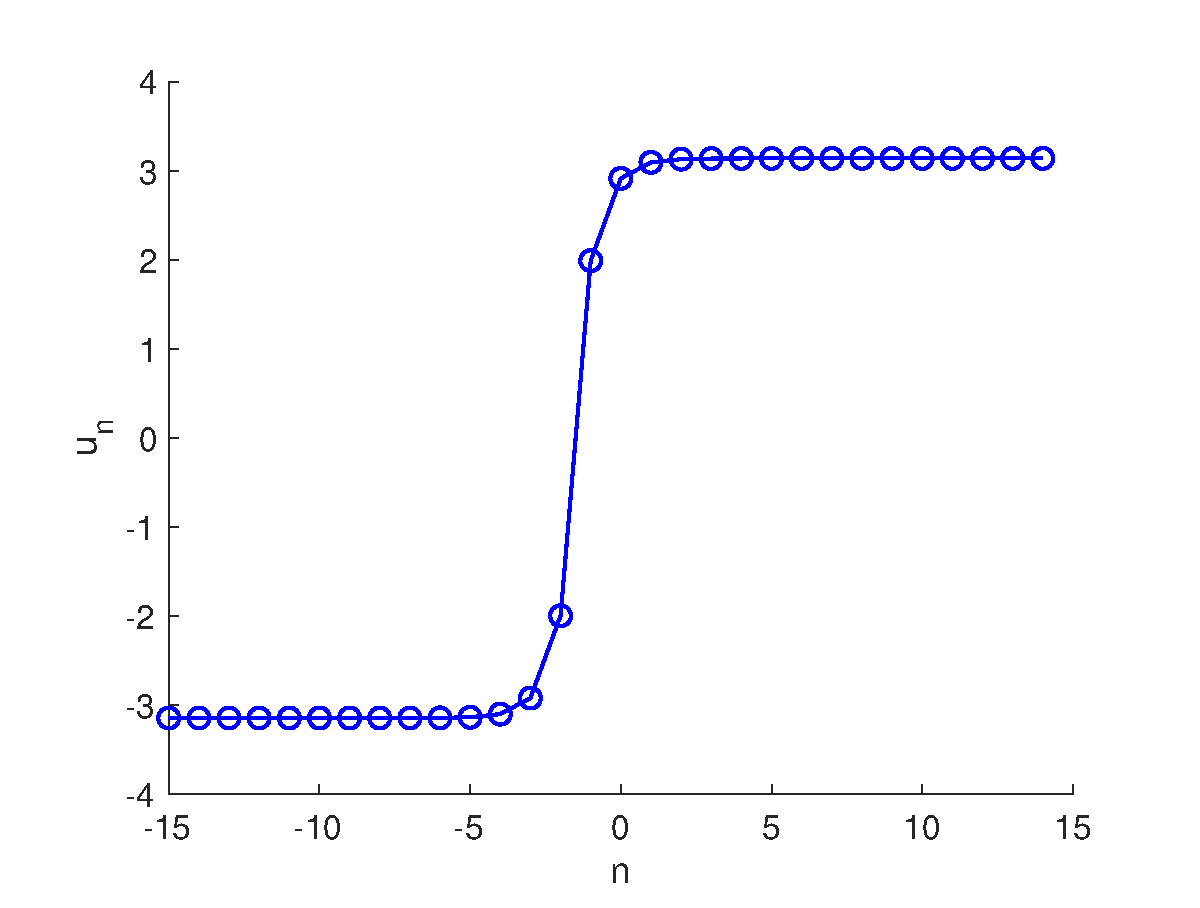
\includegraphics[width=5cm]{1kink.eps}	&
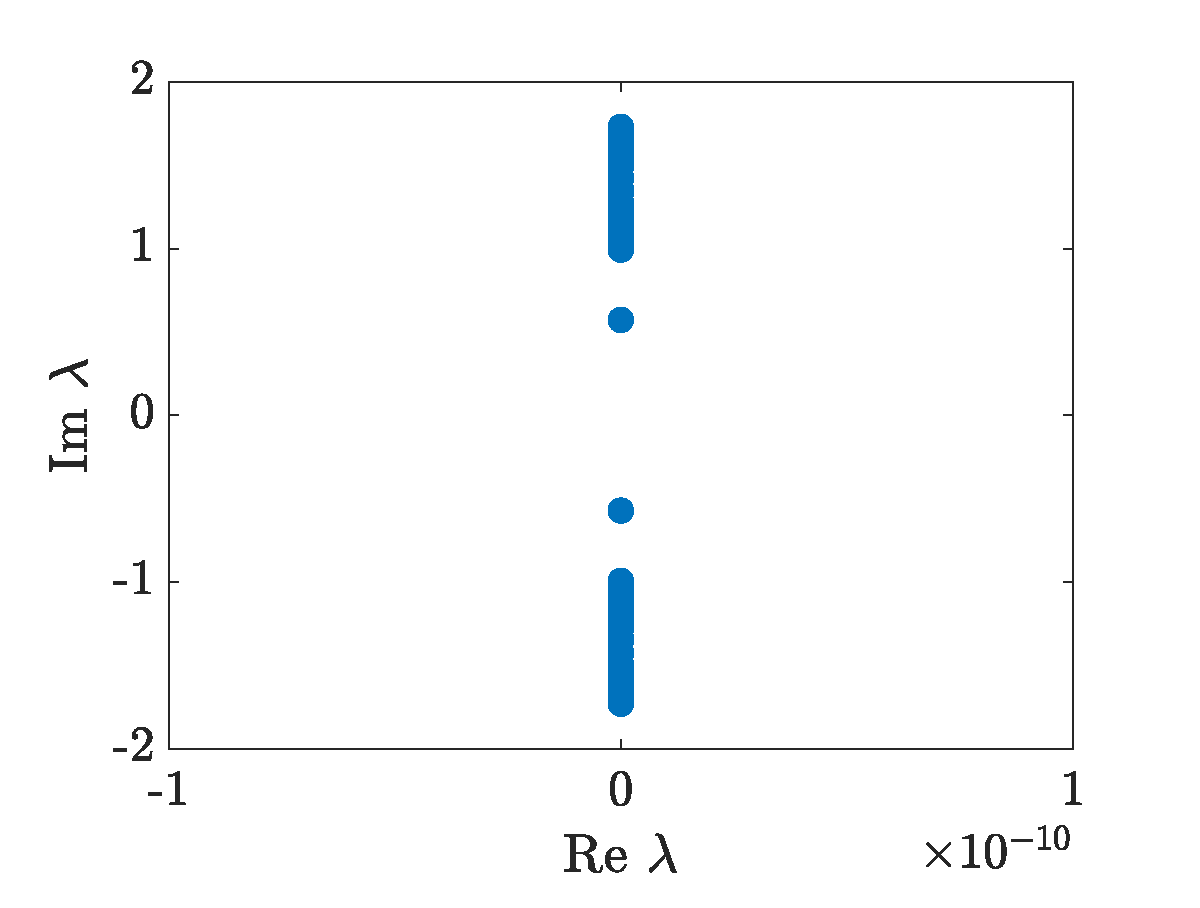
\includegraphics[width=5cm]{1kinkspectrum.eps} 
\end{tabular}
\end{center}
\caption{Primary inter-site kink (left), spectrum of primary kink (right). $d = 0.30$.}
\label{fig:kink}
\end{figure}

The continuous spectrum lies within the interval given by \cref{eq:contspec}, and the pair of Goldstone mode eigenvalues is clearly visible in the continuous spectrum gap. For approximately $d > 0.265$, there is an additional internal mode eigenvalue, known as an edge mode since it arises from the continuous spectrum (see \cite{KevrekidisWeinstein2000}*{Section 2.2}, noting that we are using $d$ in place of $d^2$ in that paper.) The eigenfunctions corresponding to the Goldstone mode and the edge mode are shown in the left and center panels of of \cref{fig:kinkeig}. The semilog plot in the right panel shows the exponential decay of the primary kink to $\pi$ and the eigenfunctions to 0 as the lattice site index $n$ increases. These decay rates are predicted to be $r^{-|n|}$ for the primary kink, and $r_0^{-|n|}$ for the eigenfuncions, where $r$ is given by \cref{eq:r} and $r_0$ (which depends on the eigenvalue) is given by \cref{eq:r0}. The decay rates computed from the least squares linear regression lines have a relative error of order $10^{-4}$ for the kink and the Goldstone mode and a relative error of $10^{-2}$ for the edge mode.

\begin{figure}[H]
	\begin{center}
	\begin{tabular}{ccc}
	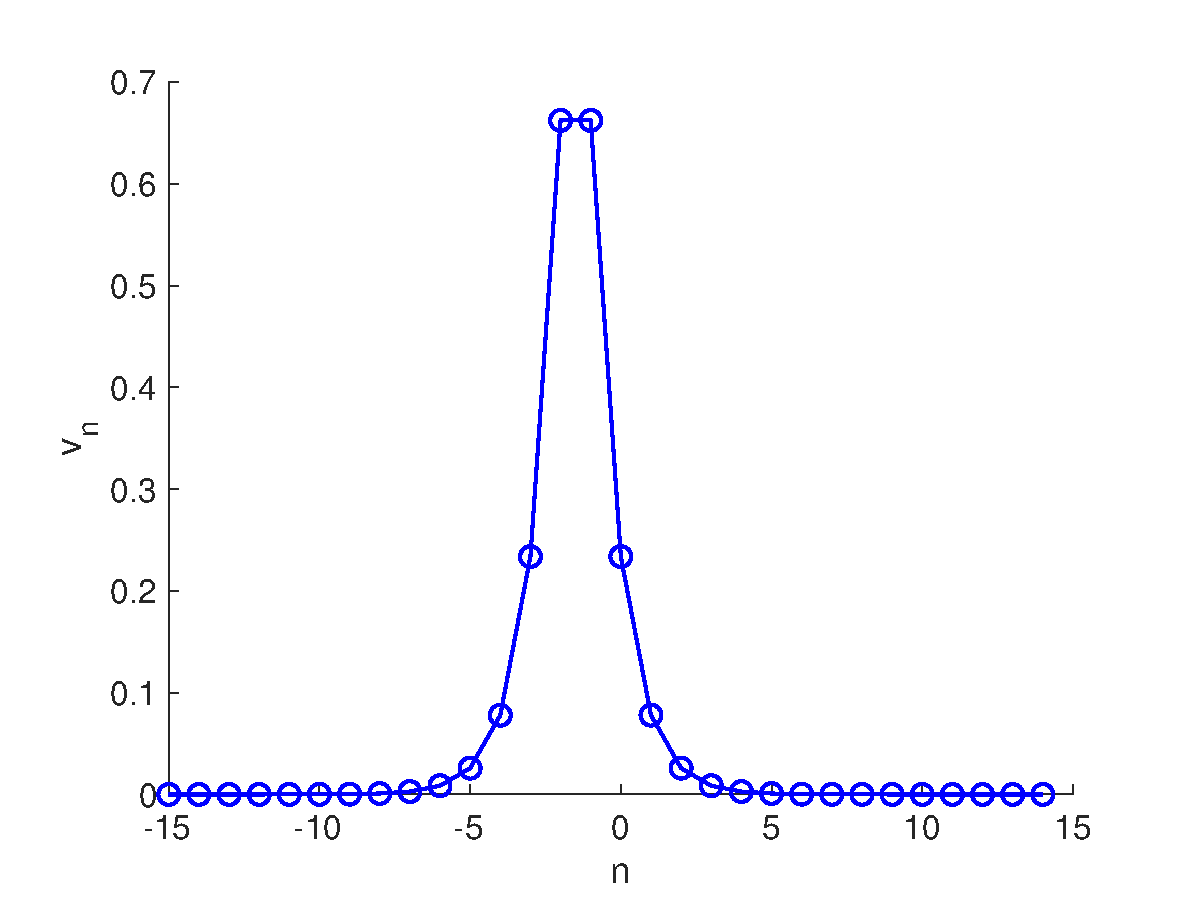
\includegraphics[width=5cm]{1kinkgoldstonemode.eps} &
	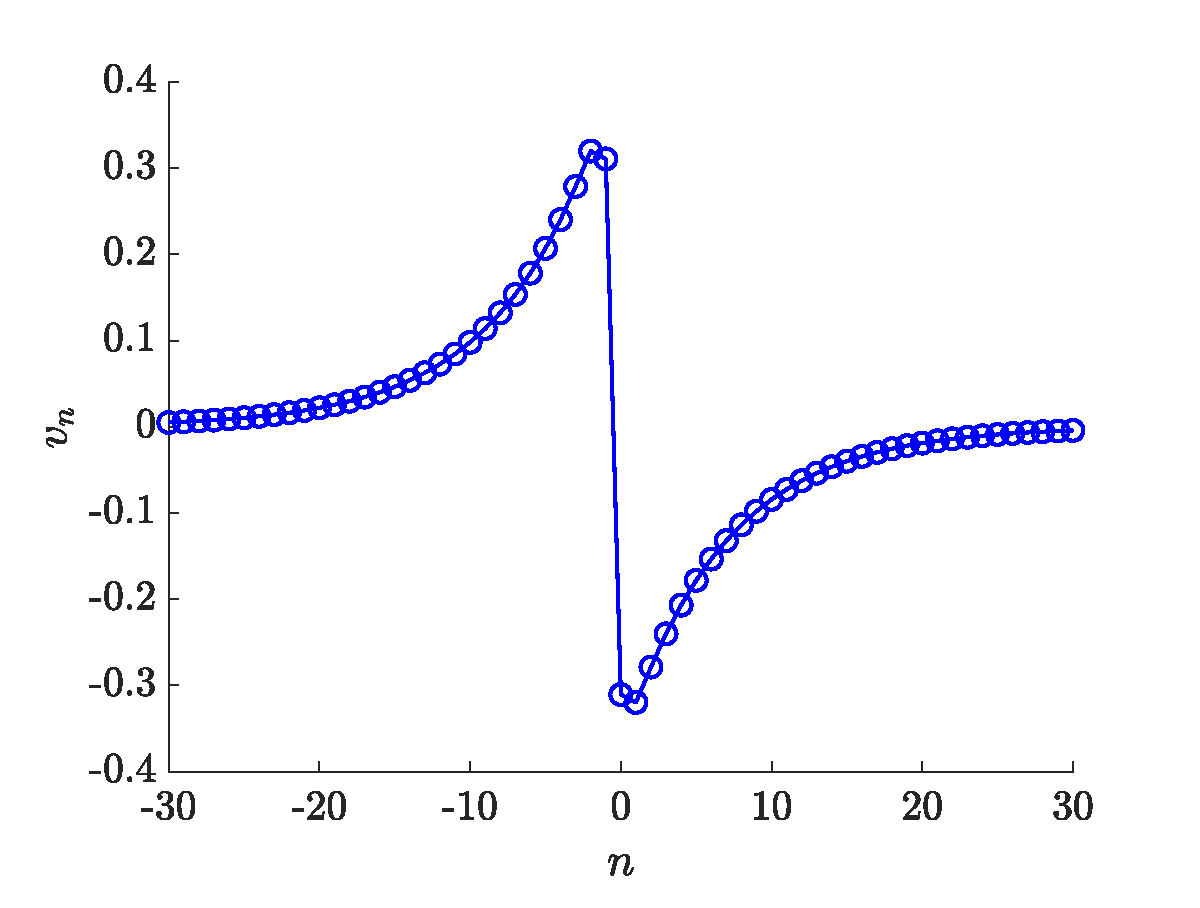
\includegraphics[width=5cm]{1kinkedgemode.eps} &
	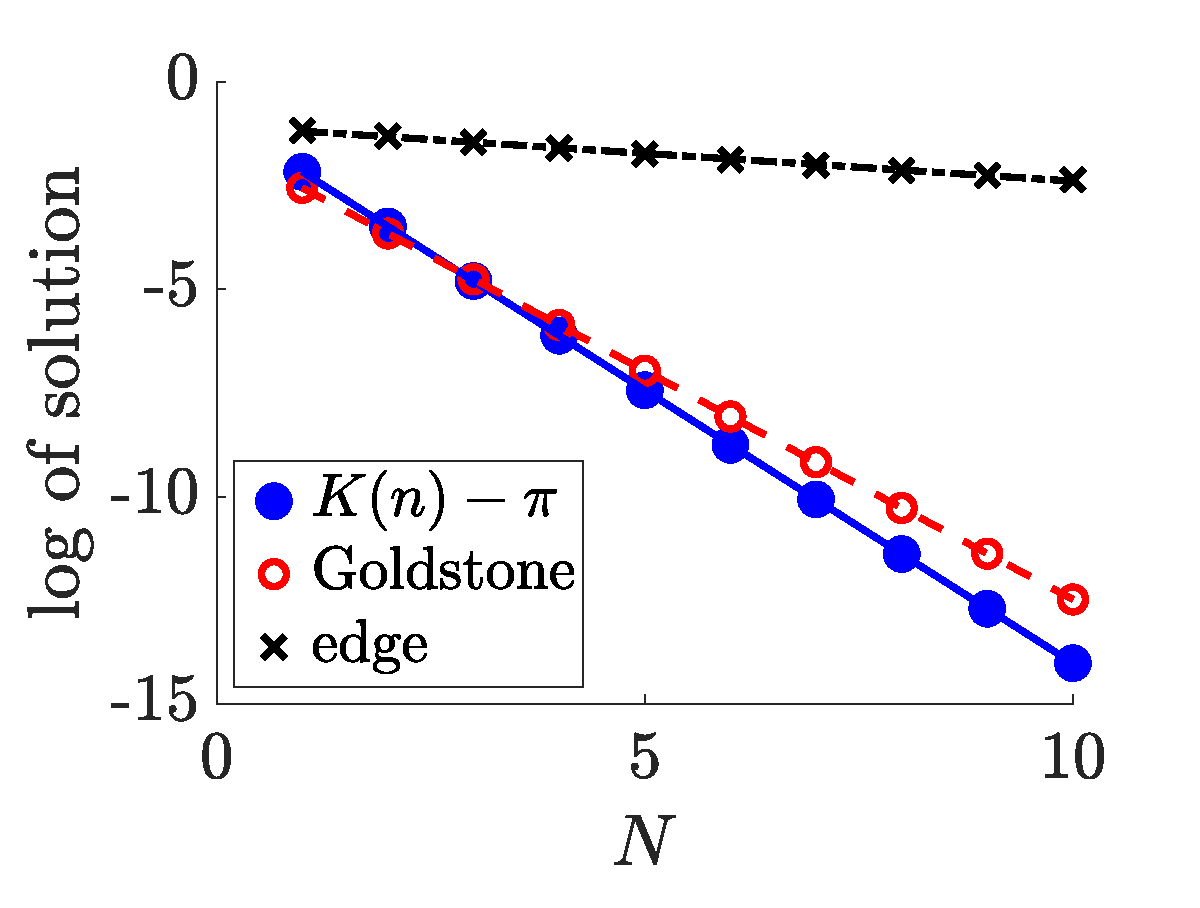
\includegraphics[width=5cm]{decayplot.eps}
	\end{tabular}
	\end{center}
	\caption{Goldstone mode eigenfunction ($\lambda = \pm 0.5718 i$, left) and edge mode eigenfunction ($\lambda = \pm 0.9941 i$, center). Semilog plot of decay of primary kink to $\pi$ and decay of Goldstone and edge modes to 0 (right) Lines are least-squares linear regressions. $d = 0.50$. }
	\label{fig:kinkeig}
\end{figure}

We construct a kink-antikink (\cref{fig:kak}, middle panel) by parameter continuation in the coupling parameter $d$ from the AC limit with AUTO. As an initial condition, we use a kink-antikink composed of two intersite kinks, which at the AC limit has the form $(\cdots, -\pi, -\pi, \pi, \pi, \dots, \pi, -\pi, -\pi, \dots )$, where there are $N_1$ sites in the middle of the solution which take the value $\pi$. The bifurcation diagram for the parameter continuation is shown in \cref{fig:SGbifdiag}. Notably, there is a turning point at a critical value $d_0$ (label 4 in the inset), where the kink-antikink does not exist for $d > d_0$. The top branch of the bifurcation diagram in \cref{fig:kak} is a kink-antikink comprising two intersite kinks, and the bottom branch is a kink-antikink comprising two on-site kinks. There is also a middle branch, which is an asymmetric kink-antikink comprising one intersite kink and one on-site kink, which meets the bottom branch at pitchfork bifurcation point at a value of $d$ slightly smaller than $d_0$. We note that the center branch of the bifurcation diagram in \cref{fig:SGbifdiag} is composed of two branches: solutions on one branch are an intersite kink followed by an on-site antikink (label 2), and solutions on the other branch are an on-site kink followed by an intersite kink (not shown in the figure). Solutions on these two branches are left-right mirror images of each other and have the same $\ell^2$ norm at the same value of $d$. Insets in the right panel of \cref{fig:SGbifdiag} show the Goldstone eigenvalue pattern for the kink-antikink solutions. Pairs of Goldstone eigenvalues collide at the origin at the two bifurcation points. The parameter continuation suggests a linear relationship between the critical value $d_0$ and the separation distance $N$, which is shown in the right panel of  \cref{fig:kak}.

\begin{figure}[H]
	\begin{center}
	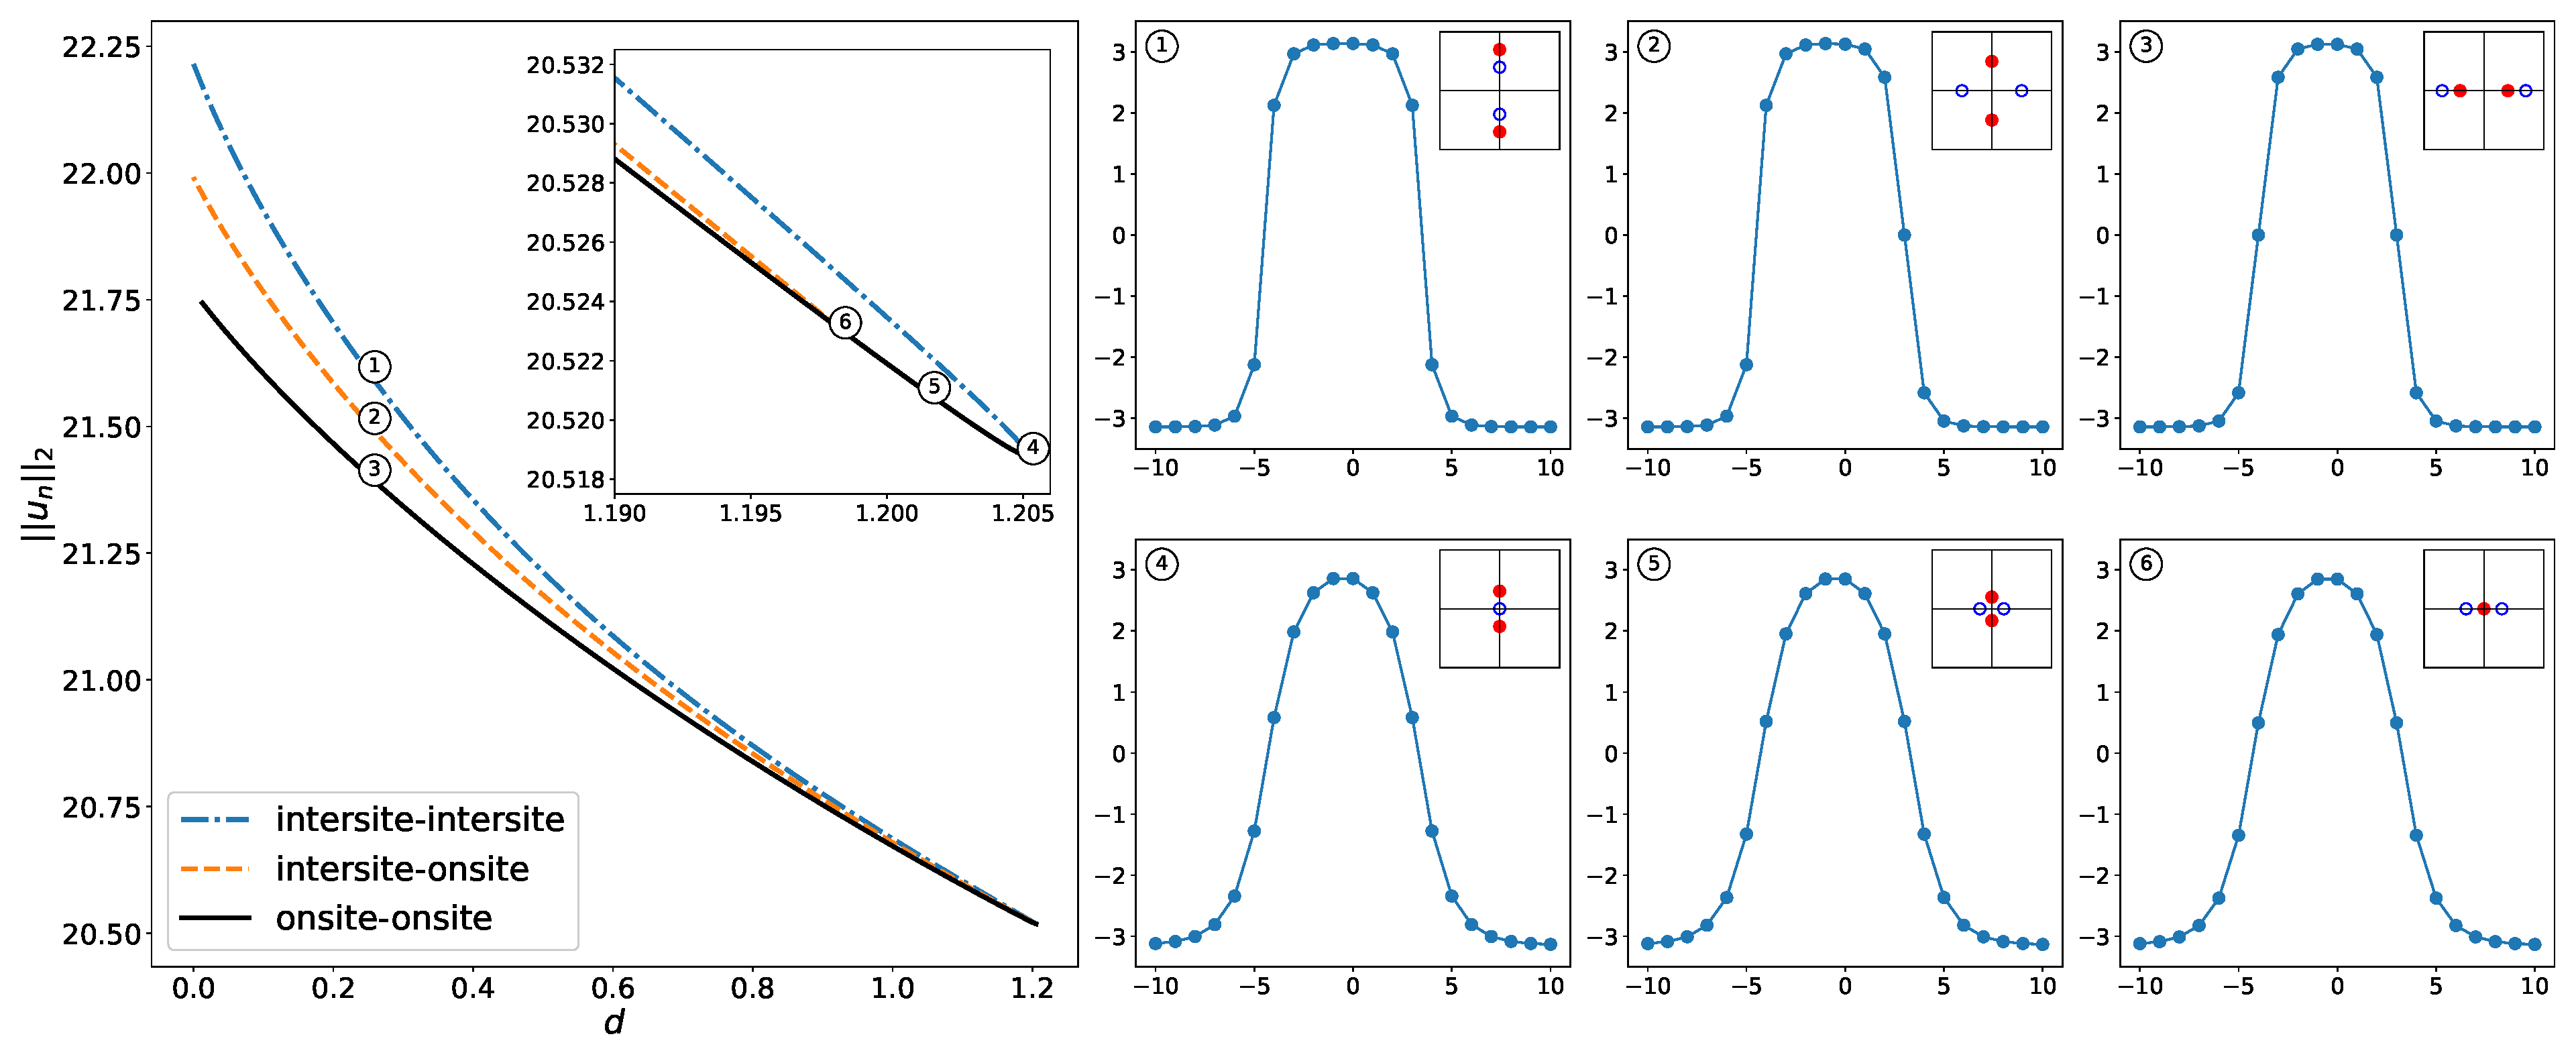
\includegraphics[width=16.5cm]{SGbifdiag.eps}
	\end{center}
	\caption{Left panel shows bifurcation diagram for kink-antikink with $N_1 = 8$, plot is of $\ell^2$ norm of solution versus coupling parameter $d$. Three branches correspond intersite-intersite, intersite-onsite, and onsite-onsite kink-antikinks. Inset details intersection points of the three braches. Right panel shows six example solutions, corresponding to labeled points on the bifurcation diagram. Insets are cartoons of Goldstone eigenvalues for these solutions; a single marker at the origin represents a double eigenvalue at 0.}
	\label{fig:SGbifdiag}
\end{figure}

\begin{figure}[H]
	\begin{center}
	\begin{tabular}{cc}
	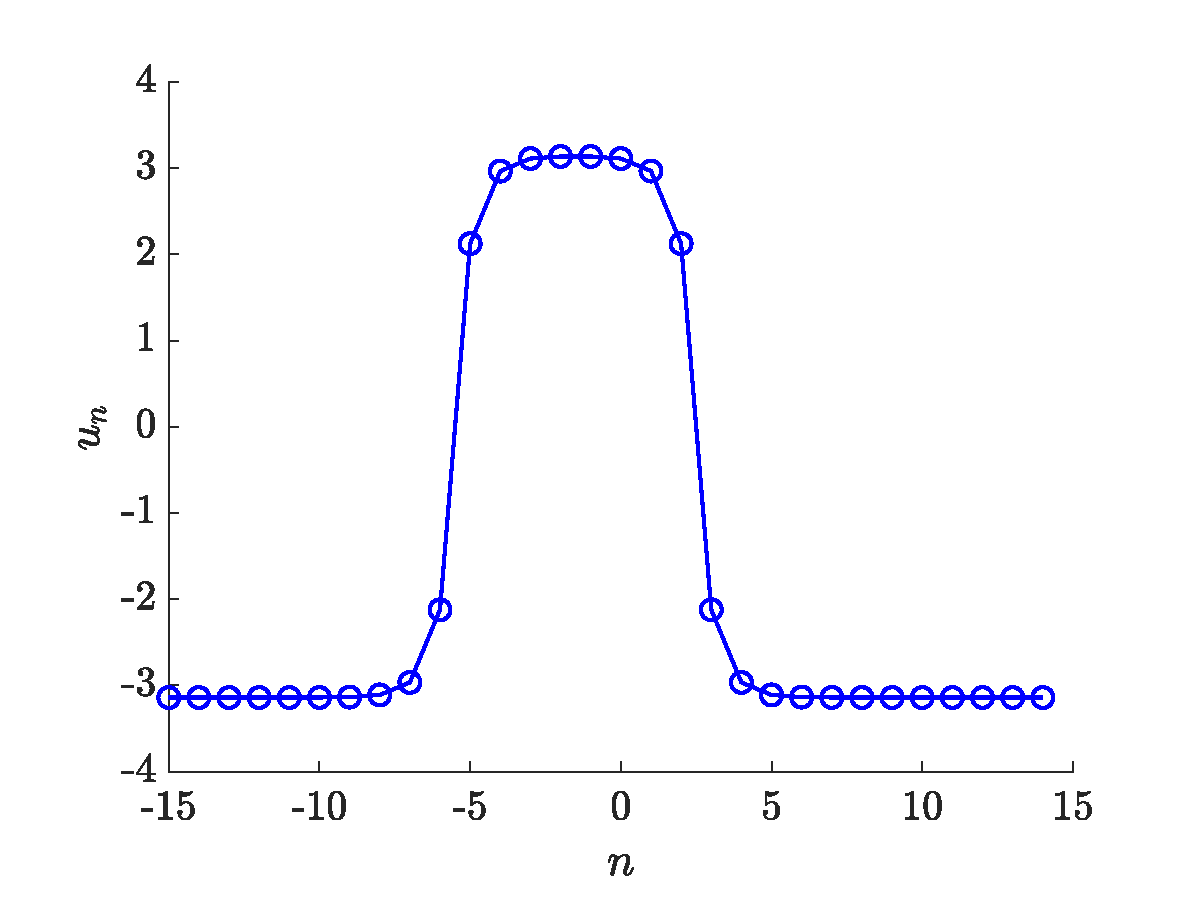
\includegraphics[width=5cm]{2kink.eps} &
	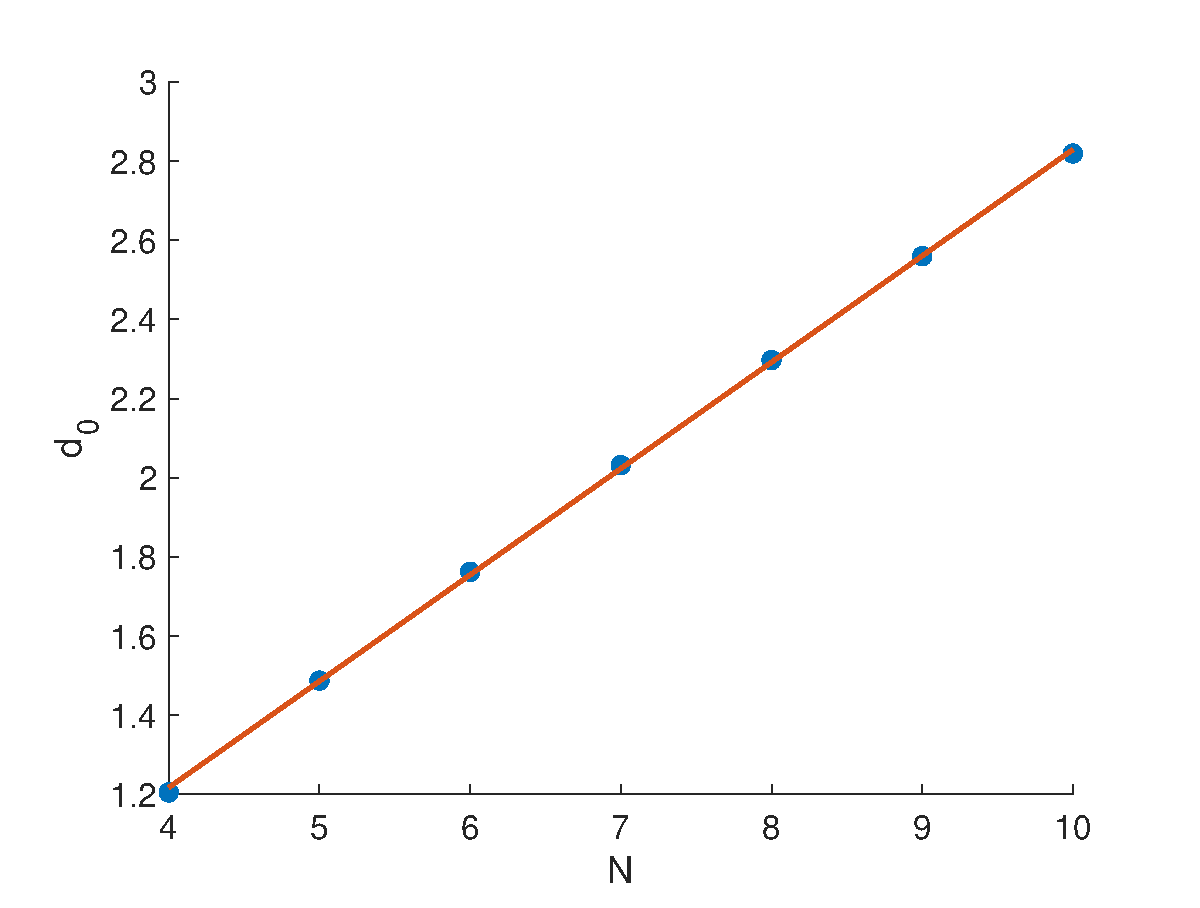
\includegraphics[width=5cm]{kakd0vsN.eps}
	\end{tabular}
	\end{center}
	\caption{Left panel shows kink-antikink solution with $N_1 = 8$ for $d = 0.5$. Right panel shows turning point $d_0$ vs $N$ for kink-antikink together with least squares linear regression line.}
	\label{fig:kak}
\end{figure}

The spectrum of the kink-antikink is similarly computed (\cref{fig:kakspec}, left panel). As predicted by \cref{th:stability}, each element of the point spectrum splits into two eigenvalues. The eigenfunctions corresponding to the split Goldstone modes resemble two copies of the Goldstone eigenfunction of the primary kink, spliced together both in-phase and out-of-phase (\cref{fig:kakspec}, center panel). A similar phenomenon occurs with the split edge mode eigenfunctions (\cref{fig:kakspec}, right panel).

\begin{figure}[H]
	\begin{center}
	\begin{tabular}{ccc}
	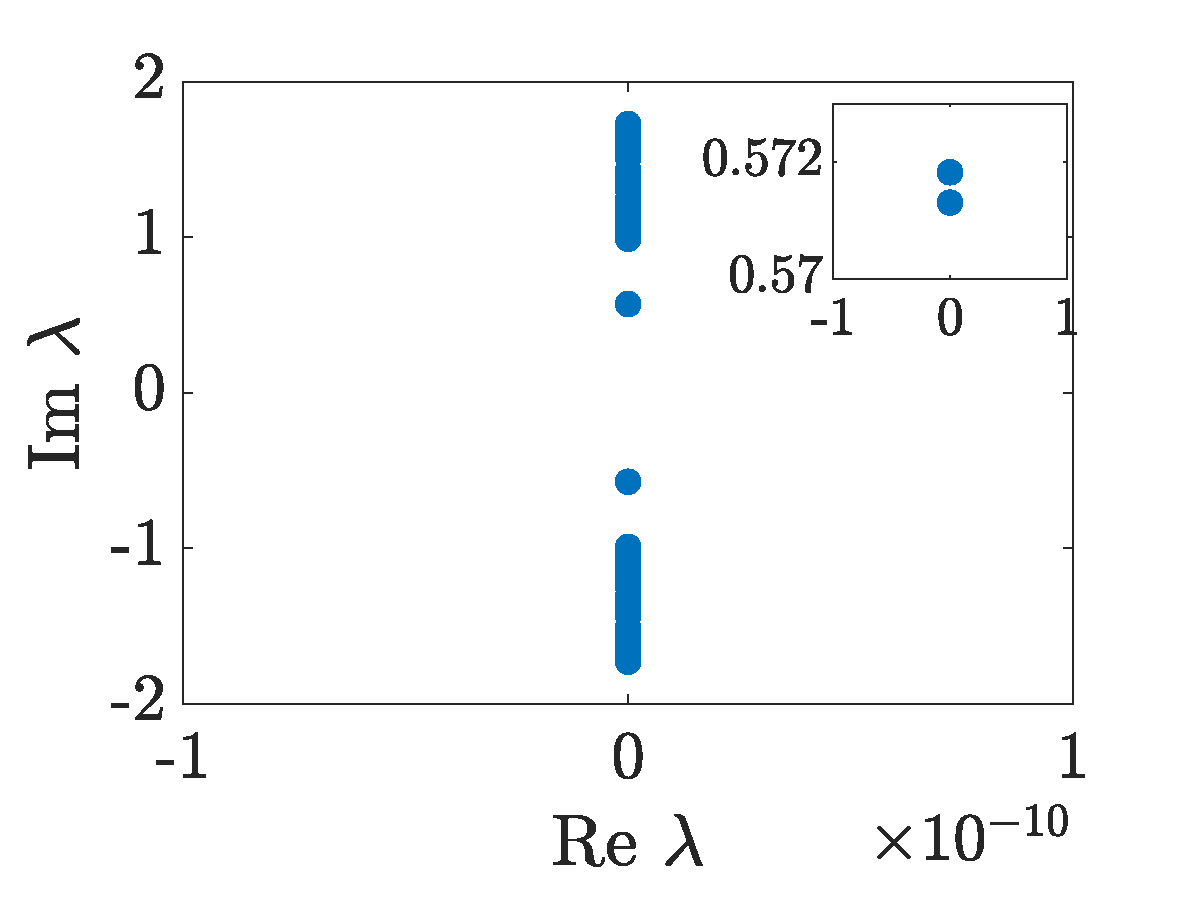
\includegraphics[width=5cm]{kak50_8spec.eps}	&
	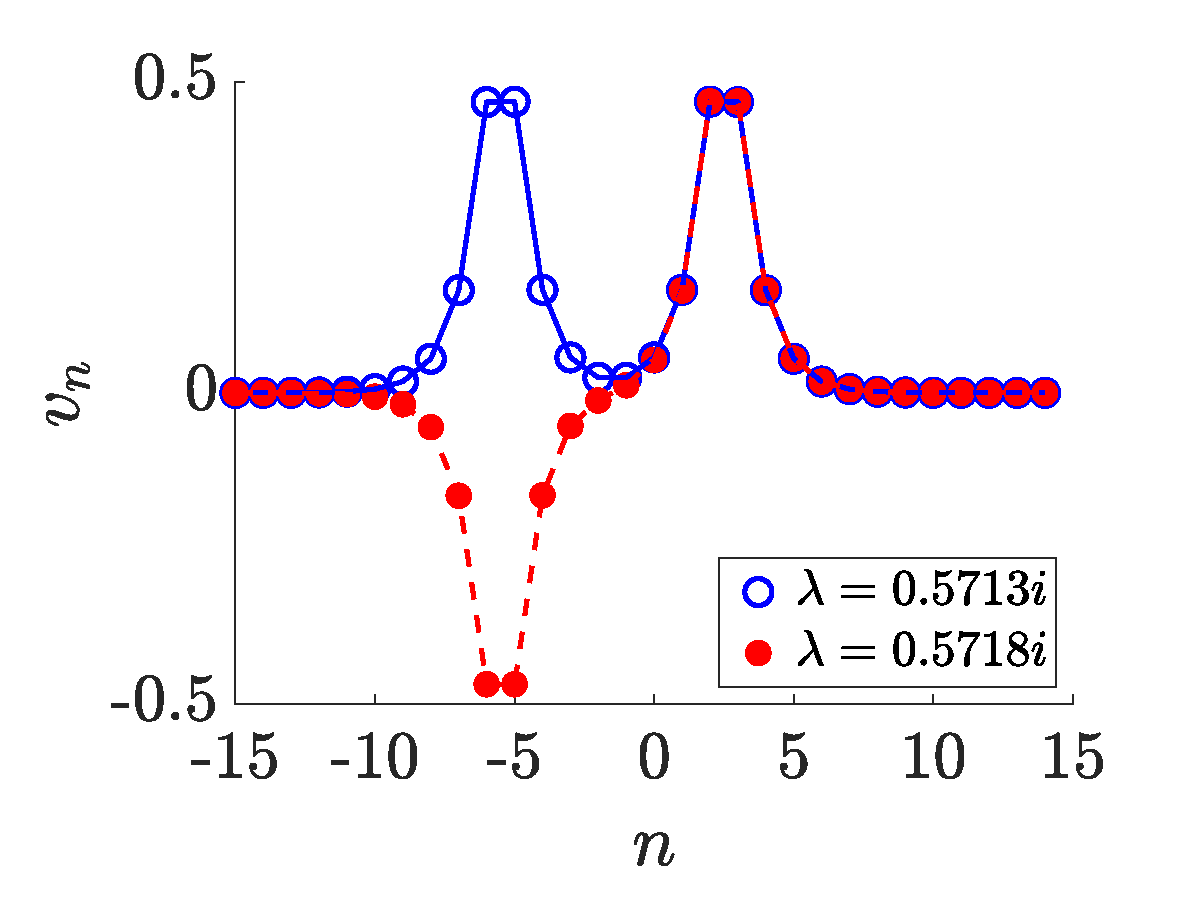
\includegraphics[width=5cm]{kak50_8goldstone.eps} &
	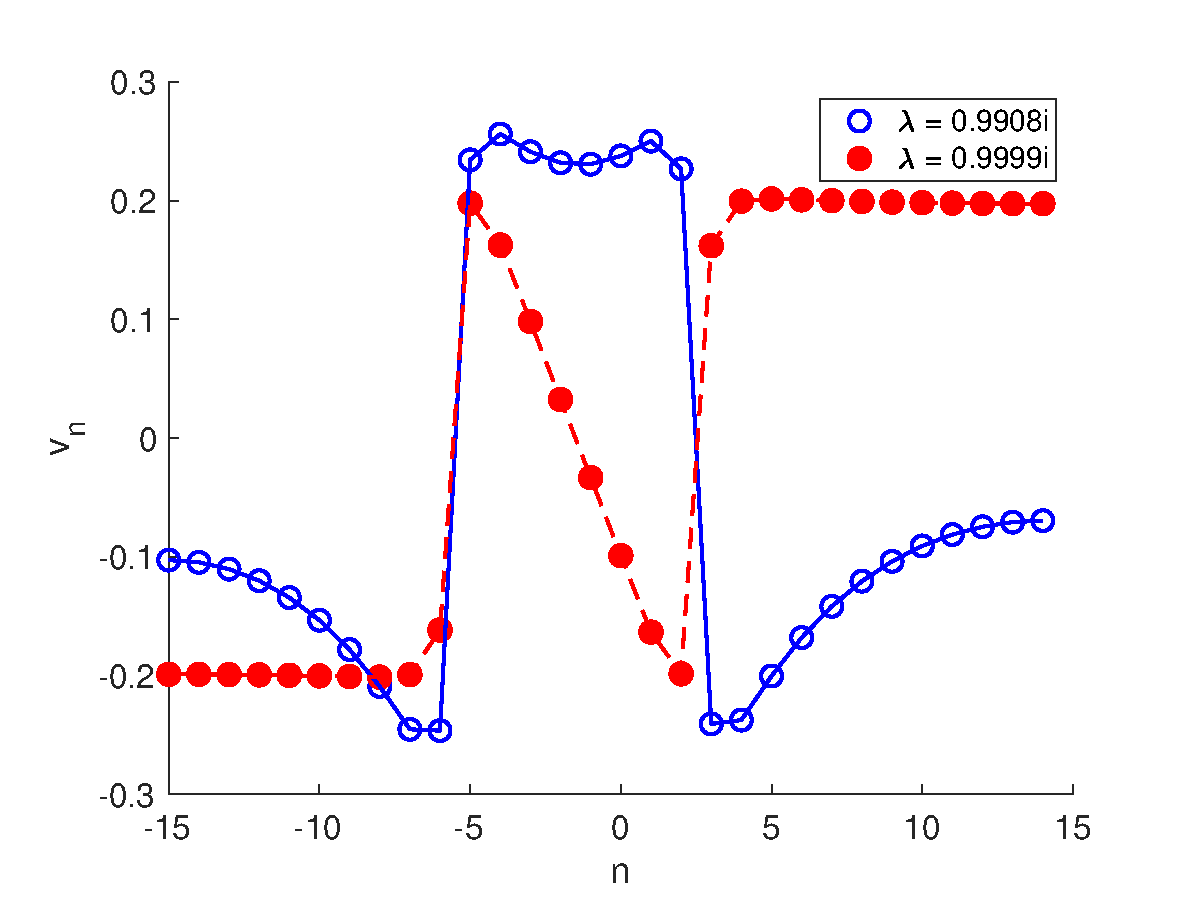
\includegraphics[width=5cm]{kak50_8edge.eps}
	\end{tabular}
	\end{center}
	\caption{Left panel shows spectrum of kink-antikink, with inset showing splitting of Goldstone mode. Edge mode is also split (not shown). Center panel shows eigenfunctions corresponding to split Goldstone modes. Right panel shows eigenfunctions corresponding to split edge modes. $d = 0.5$, $N = 4$.}
	\label{fig:kakspec}
\end{figure}

We can compare the eigenvalues obtained from numerical computation with those predicted by the \cref{corr:m23}. The left panel of \cref{fig:kakeigerror} plots the log of the relative error of the two Goldstone eigenvalues vs. the separation distance $N$. The slope of the least square linear regression line suggests that this error is order $\mathcal{O}(r^{-2N})$. The right panel of \cref{fig:kakeigerror} plots the log of the relative error of the two Goldstone eigenvalues vs. the coupling parameter $d$. For intermediate values of d, the relative error is less than $10^{-3}$. The error is a minimum for approximately $d = 0.2$, and increases with increasing $d$. (See \cite{Parker2020}*{Figure 4} for a similar error plot for eigenvalues associated with double pulses in the DNLS equation.) Since the results of the \cref{th:stability} are not uniform in $d$, i.e. they hold for sufficiently large $N$ once $d$ has been chosen, we do not expect to have a nice relationship between the relative error and $d$.

\begin{figure}[H]
	\begin{center}
	\begin{tabular}{cc}
	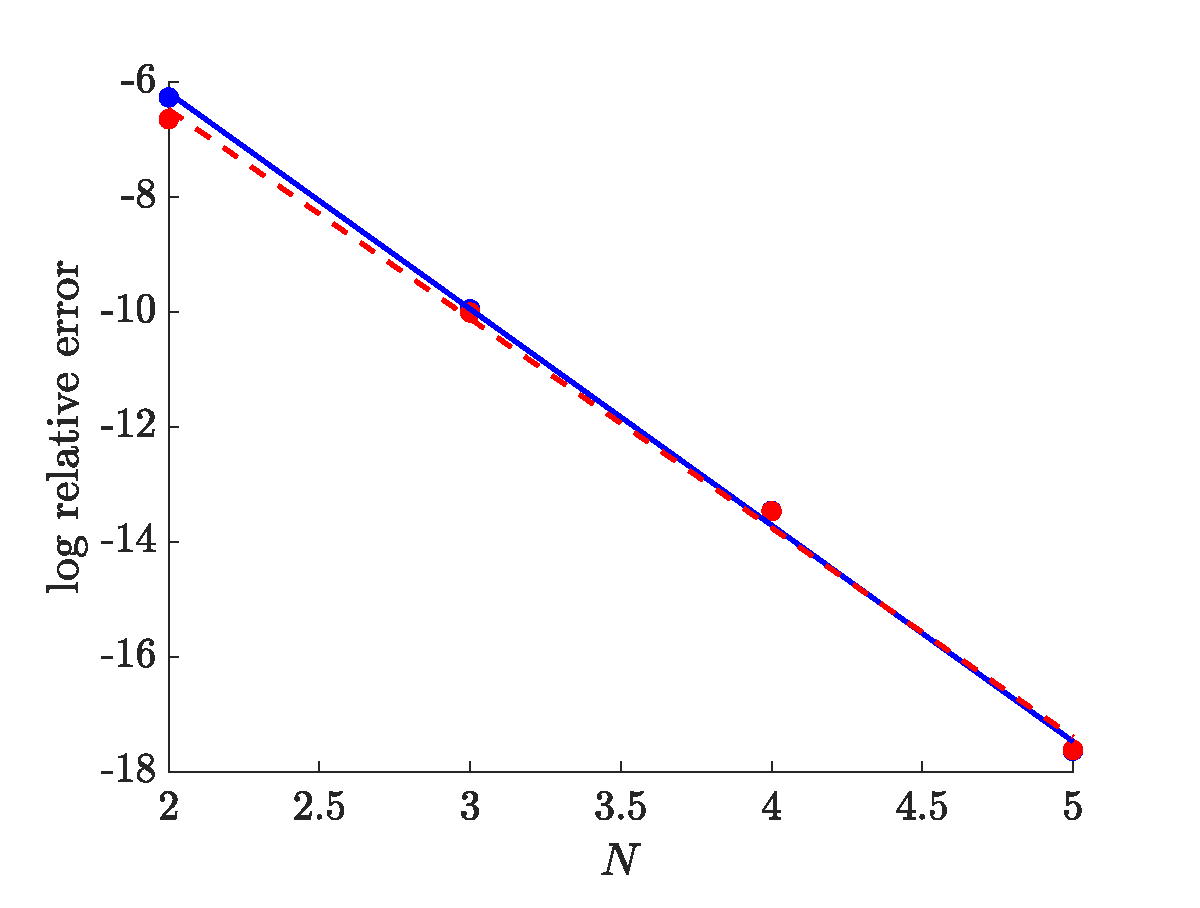
\includegraphics[width=5cm]{goldstoned025relerror.eps} &
	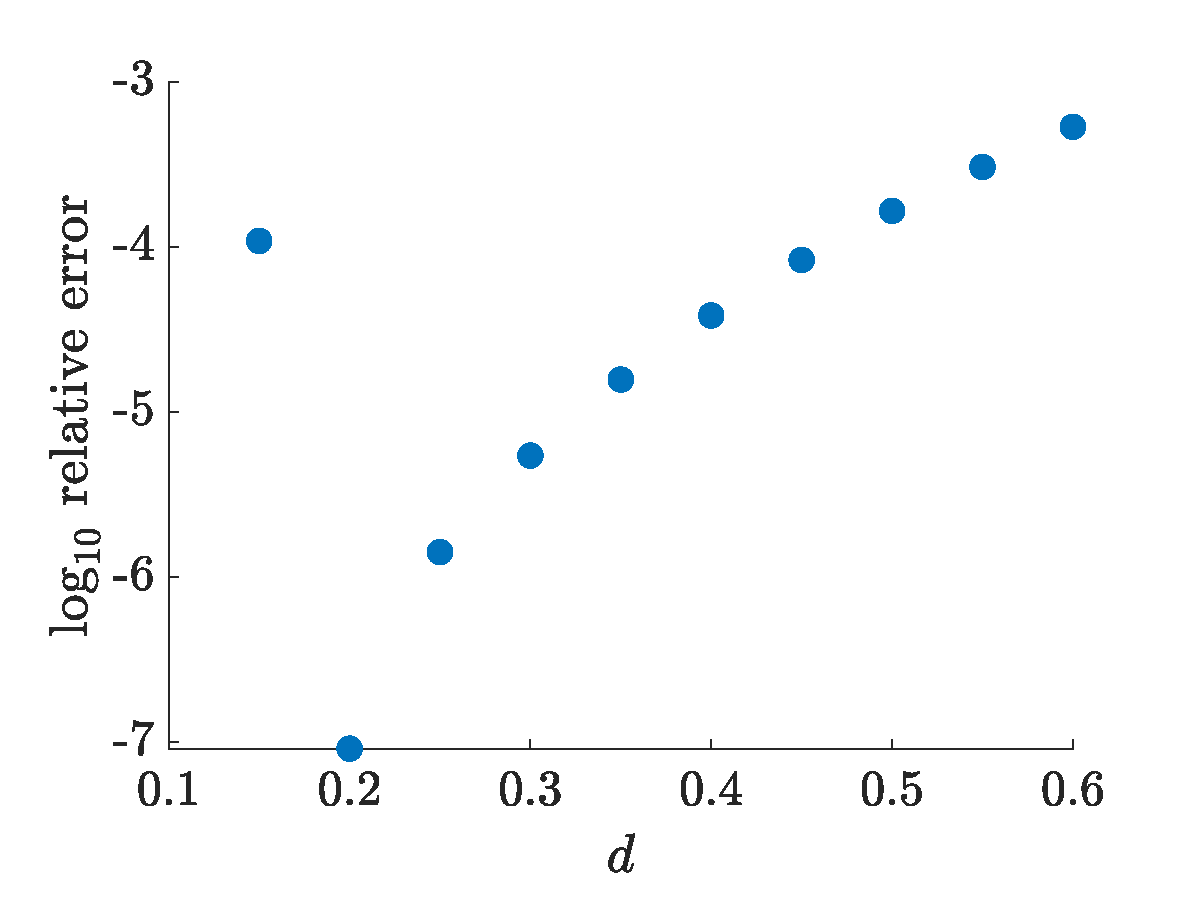
\includegraphics[width=5cm]{goldstoneN4relativeerror.eps}
	\end{tabular}
	\end{center}
	\caption{Left panel shows log of relative error in eigenvalue computation vs. $N$ for the two Goldstone eigenvalues for kink-antikink with $d = 0.25$ together with least square linear regression lines. Blue dots and blue solid line are one Goldstone eigenvalue, red dots and red dashed line are the other Goldstone eigenvalue. Right panel shows $log_{10}$ of relative error in eigenvalue computation vs. $d$ for the two Goldstone eigenvalues for kink-antikink with $N = 4$.} 
	\label{fig:kakeigerror}
\end{figure}

We can obtain similar results for higher order multi-kinks. An example of a 3-component multi-kink is shown in the left panel of \cref{fig:3p}. We can again compare the eigenvalue obtained from numerical computation with those predicted by \cref{corr:m23}. The right panel of \cref{fig:3p} shows the relative error of the eigenvalues computations for the three Goldstone eigenvalues.

\begin{figure}[H]
	\begin{center}
	\begin{tabular}{cc}
	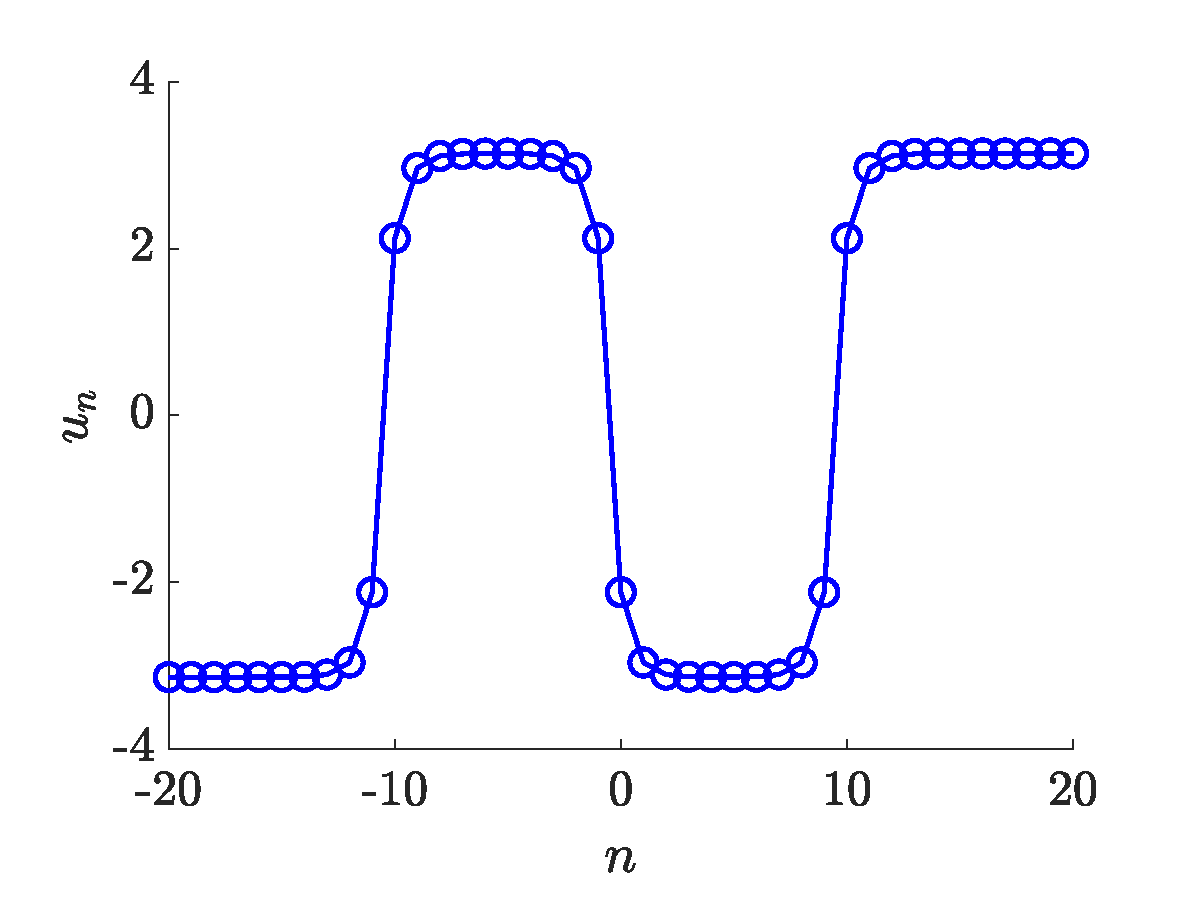
\includegraphics[width=5cm]{3kink.eps} &
	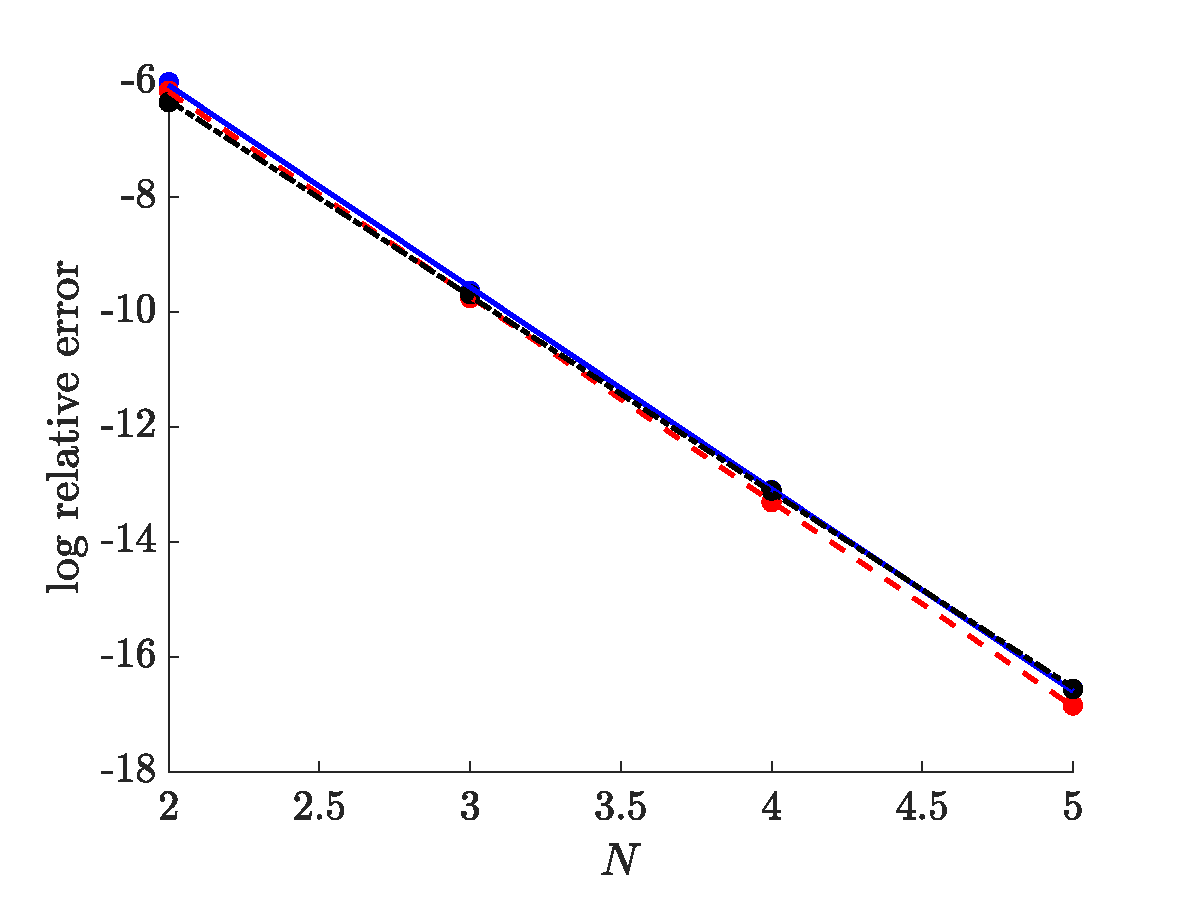
\includegraphics[width=5cm]{goldstone3prelerror.eps}
	\end{tabular}
	\end{center}
	\caption{Left panel shows 3-component multi-kink (kink-antikink-kink) with $N_1 = N_2 = 8$ and $d = 0.25$. Right panel shows log of relative error in eigenvalue computation vs. $N$ for the three Goldstone eigenvalues for 3-component multi-kink with $N_1 = N_2 = 2N$ and $d = 0.25$. Lines are least square linear regression lines.} 
	\label{fig:3p}
\end{figure}

\noi In addition, for the sine-Gordon equation, we can have generalized multi-kink solutions in which each kink or anti-kink in the sequence connects two adjacent saddle equilbria (see \cref{rem:SGmulitkinks}). An example of a kink-kink is shown in \cref{fig:kk50}. The spectrum is almost identical to that of the kink-antikink with the same parameters \cref{fig:kakspec}.
\begin{figure}[H]
	\begin{center}
	\begin{tabular}{cc}
	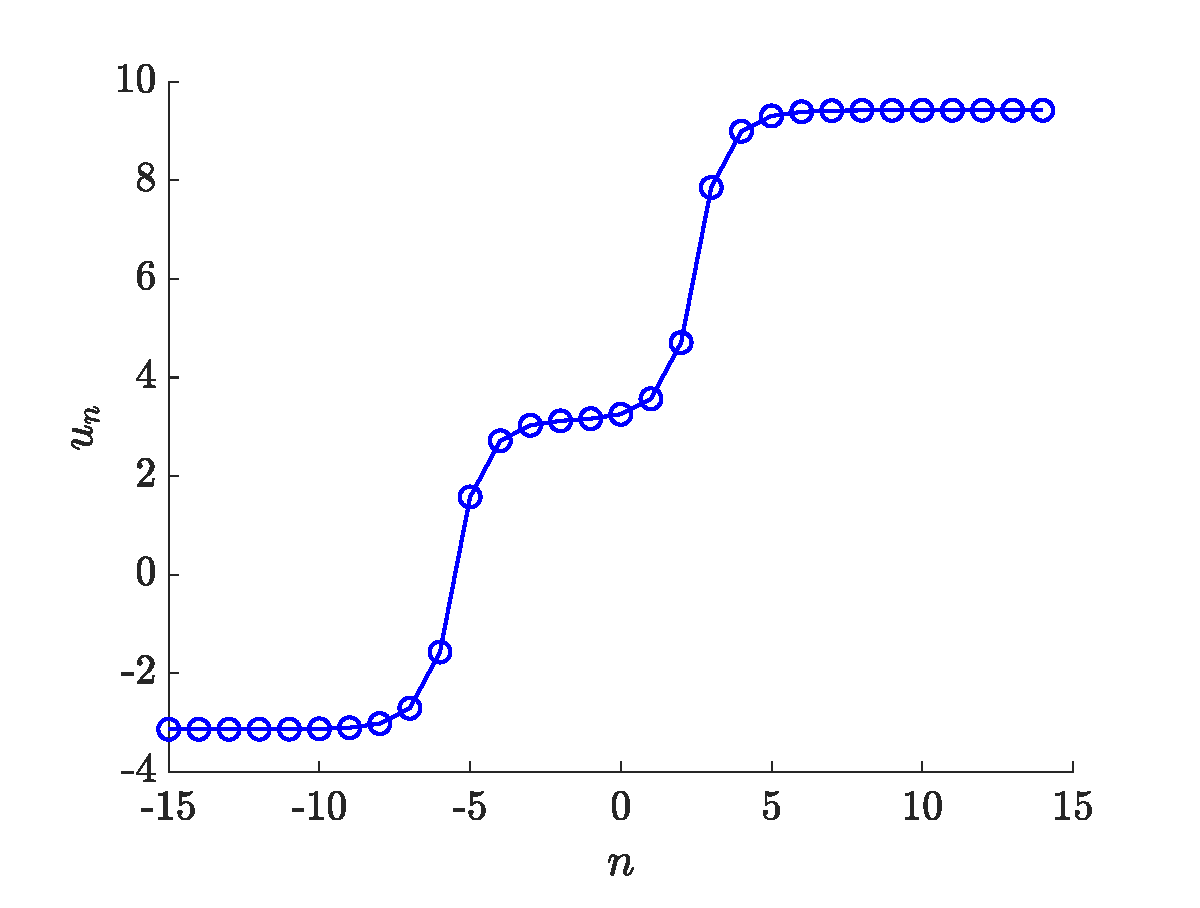
\includegraphics[width=5cm]{kk50.eps} &
	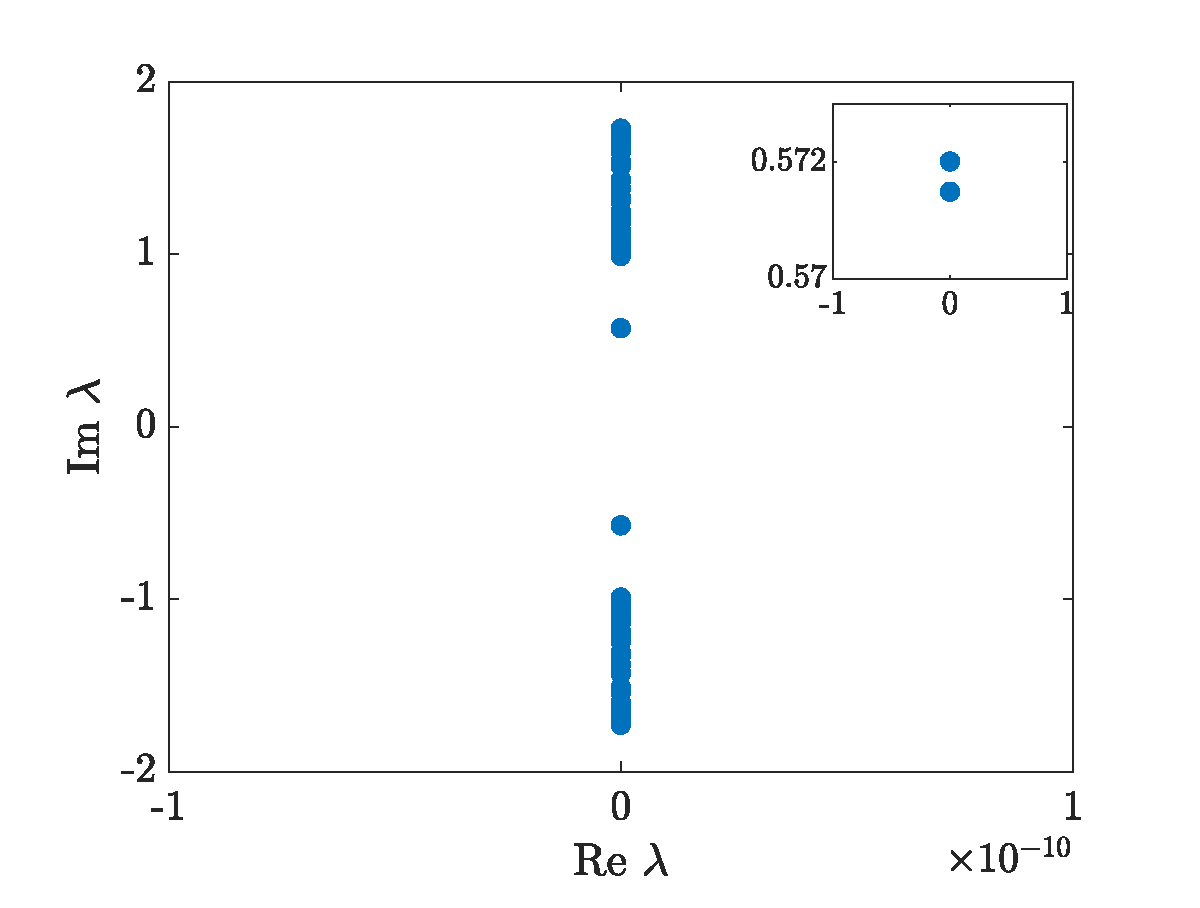
\includegraphics[width=5cm]{kk50spec.eps}
	\end{tabular}
	\end{center}
	\caption{Left panel shows kink-kink solution with $N_1 = 8$. Right panel shows spectrum of kink-antikink, with inset showing splitting of Goldstone mode. Edge mode is also split (not shown). $d = 0.25$. }
	\label{fig:kk50}
\end{figure}

Finally, we perform timestepping simulations on perturbations of the primary kink. Since the eigenvalues are imaginary, we expect to see oscillatory behavior whose form is determined by the shape of the corresponding eigenfunction. For a kink or multi-kink, we will refer to the two nodes which are closest to (and symmetric about) 0 as the central nodes (these are nodes -1 and 0 in \cref{fig:kink}). The left and central panels of \cref{fig:kinktimestep} shows the oscillatory behavior that results when the central nodes of the kink are perturbed in the same direction by 0.1. This perturbation follows the shape of the Goldstone eigenfunction, and the frequency of oscillations is given by the Goldstone eigenvalue, with a relative error of less than $10^{-2}$. Since the two central nodes perturb in the same direction, we will call these in-phase vibrations. The right panel of \cref{fig:kinktimestep} shows the oscillatory behavior that results when the central nodes of the kink are perturbed in the opposite direction by 0.1. This perturbation follows the shape of the edge mode eigenfunction, and the frequency of oscillations is given by the edge mode eigenvalue, with a relative error of less than $10^{-2}$. Since the two central nodes perturb in opposite directions, we will call these out-of-phase vibrations.

\begin{figure}[H]
	\begin{center}
	\begin{tabular}{ccc}
	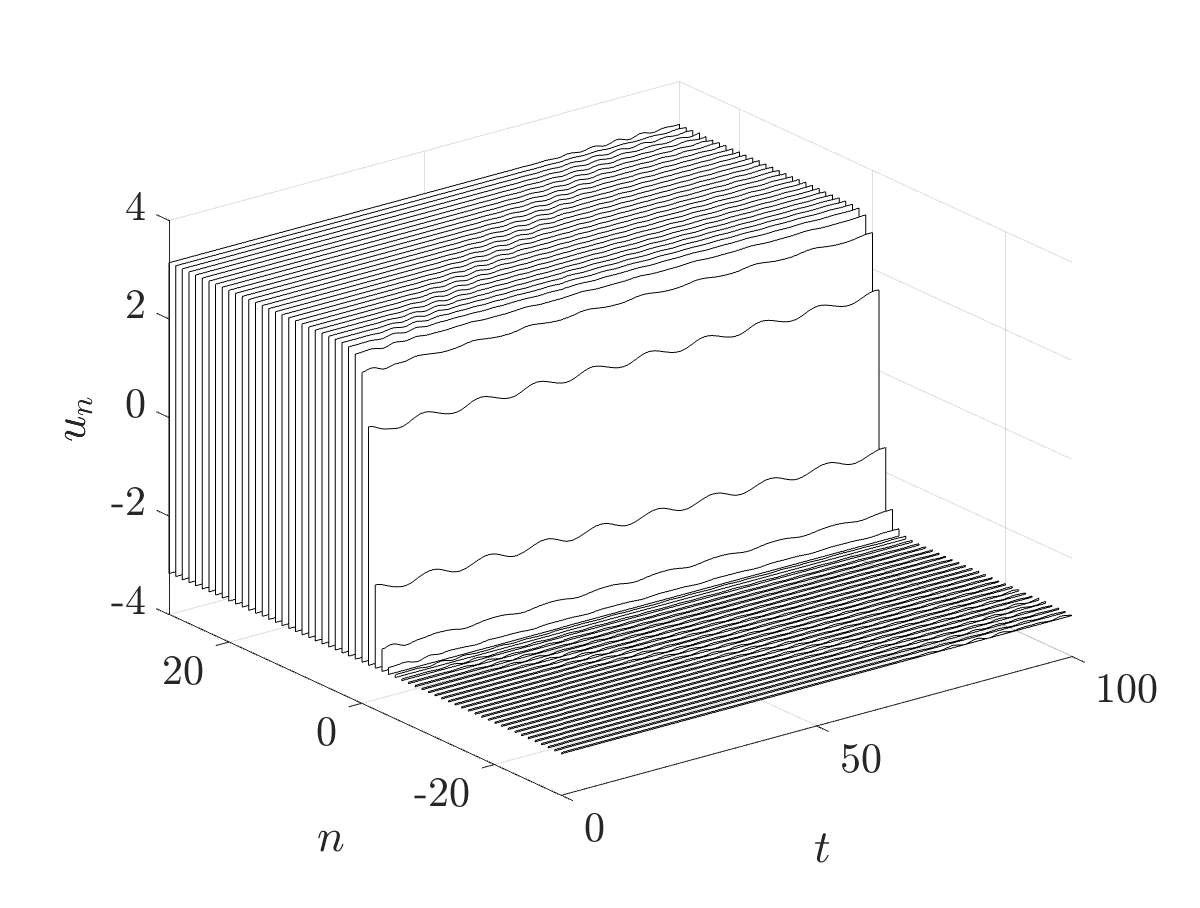
\includegraphics[width=5cm]{kinkwaterfall1.eps} &
	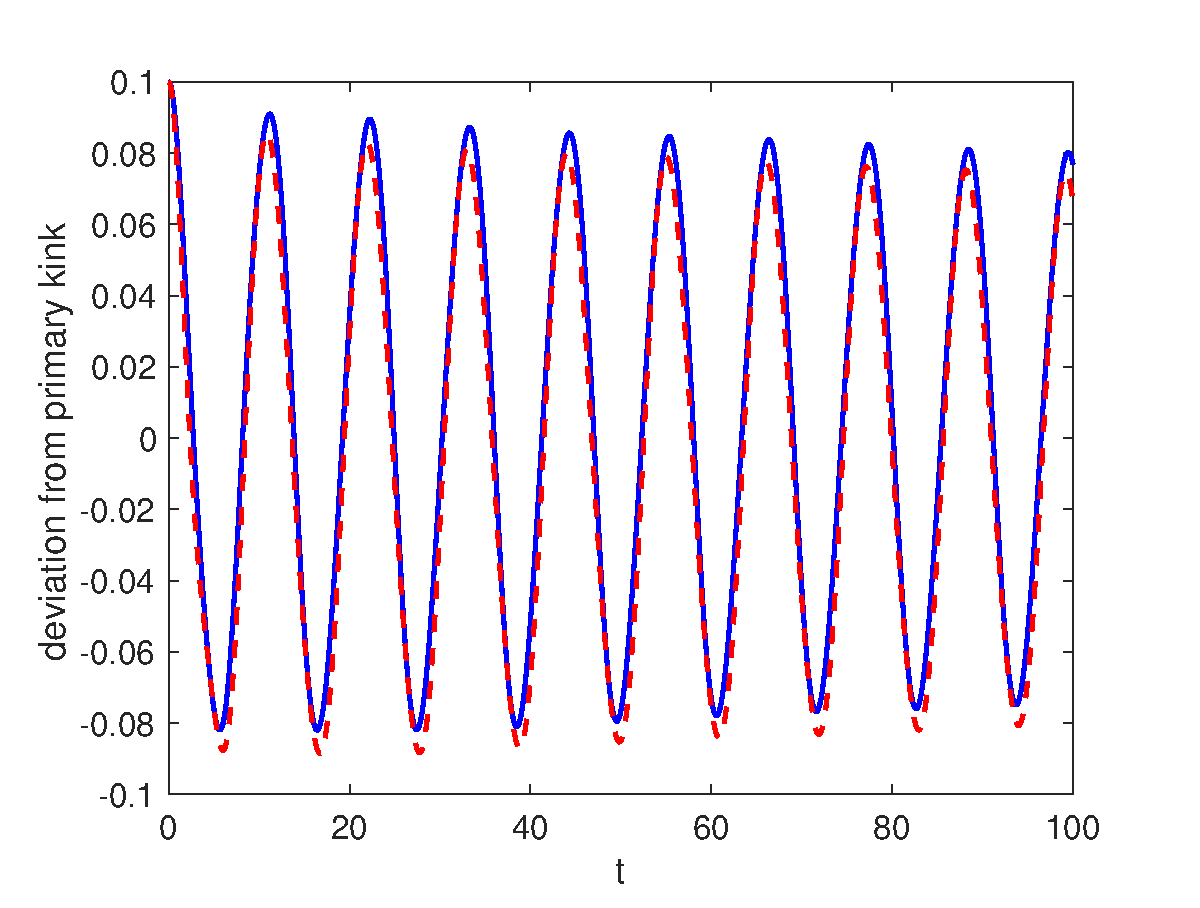
\includegraphics[width=5cm]{kinkoscgoldstone.eps} &
	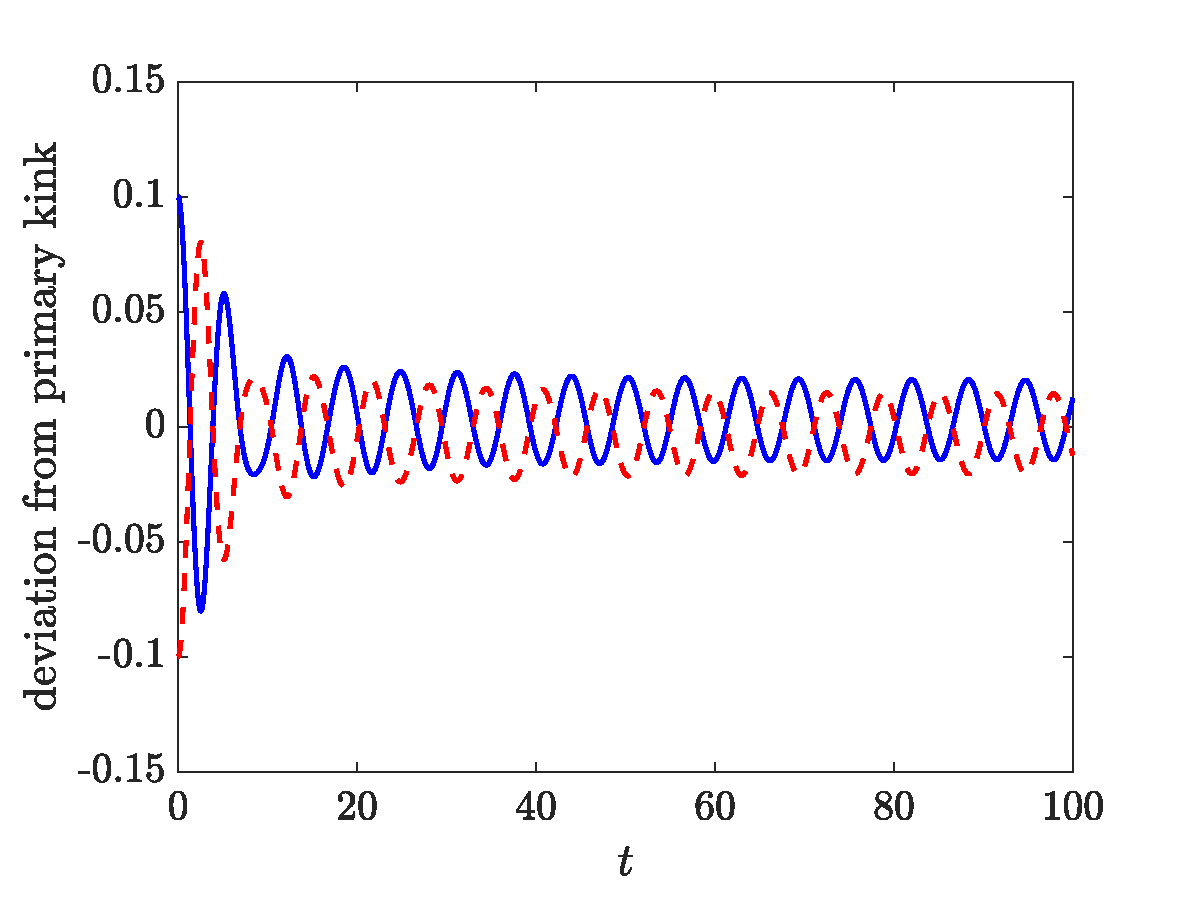
\includegraphics[width=5cm]{kinkoscedge.eps}
	\end{tabular}
	\end{center}
	\caption{Left panel shows timestepping of perturbation of primary kink solution, where two central nodes of kink are perturbed by 0.1 in same direction. Center and right panels shows difference between perturbed solution and kink for the two central nodes for perturbation of central nodes in same direction (center) and opposite direction (right) by 0.1. Two central nodes are shown in blue solid and red dotted lines. $N=200$ grid points for kink, $d = 0.70$, timestepping using 4th order Runge-Kutta method with step size 0.04. Goldstone mode eigenvalue is $0.40703i$, edge mode eigenvalue is $0.99618i$.
	} 
	\label{fig:kinktimestep}
\end{figure}

For certain values of the coupling parameter $d$, there will be resonance between the Goldstone mode and the continuous spectrum, which will cause the oscillations to decay (\cref{fig:kinktimestepresonance}, contrast with center panel of \cref{fig:kinktimestep}). This occurs when $2 \lambda$ is contained in the continuous spectrum band, where $\lambda$ is the Goldstone eigenvalue.

\begin{figure}[H]
	\begin{center}
	\begin{tabular}{cc}
	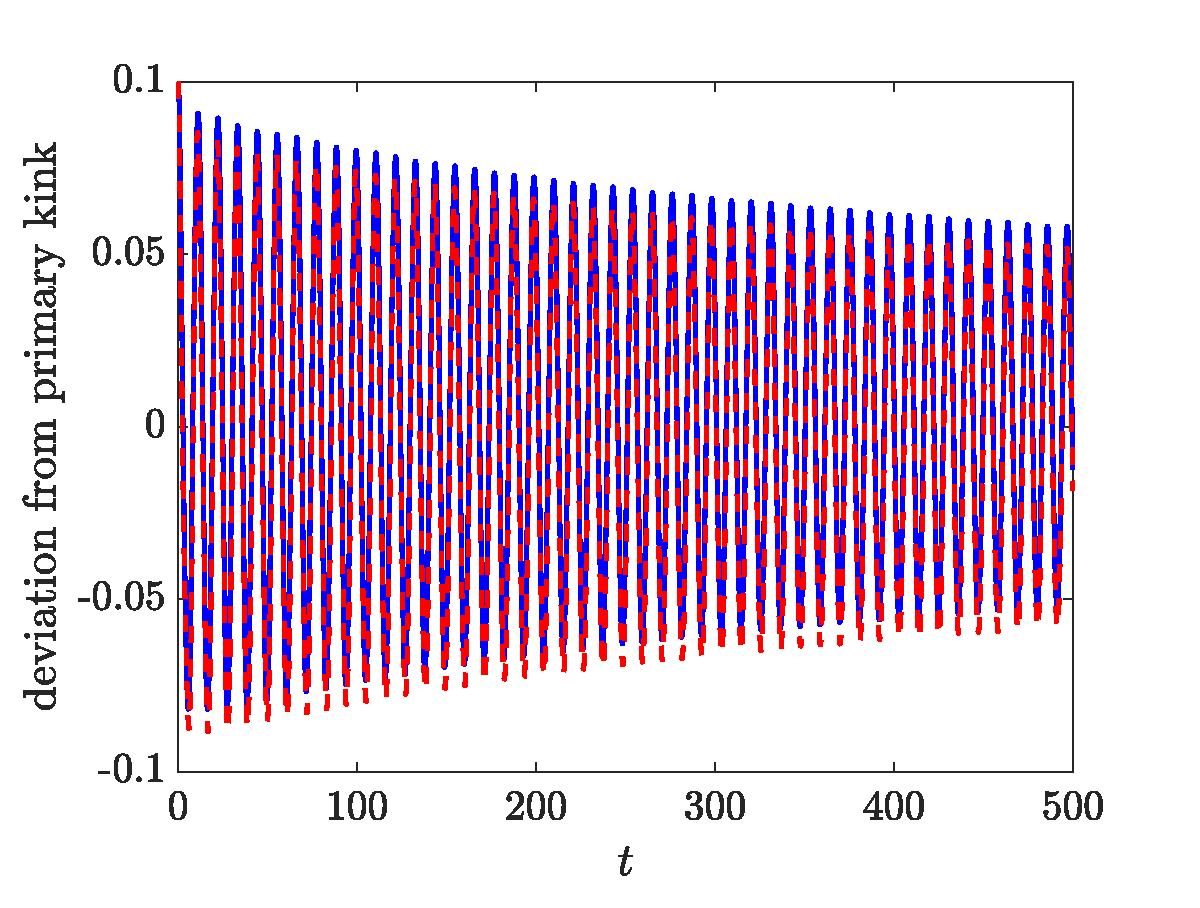
\includegraphics[width=6cm]{kinkoscgoldstonek50N200.eps} &
	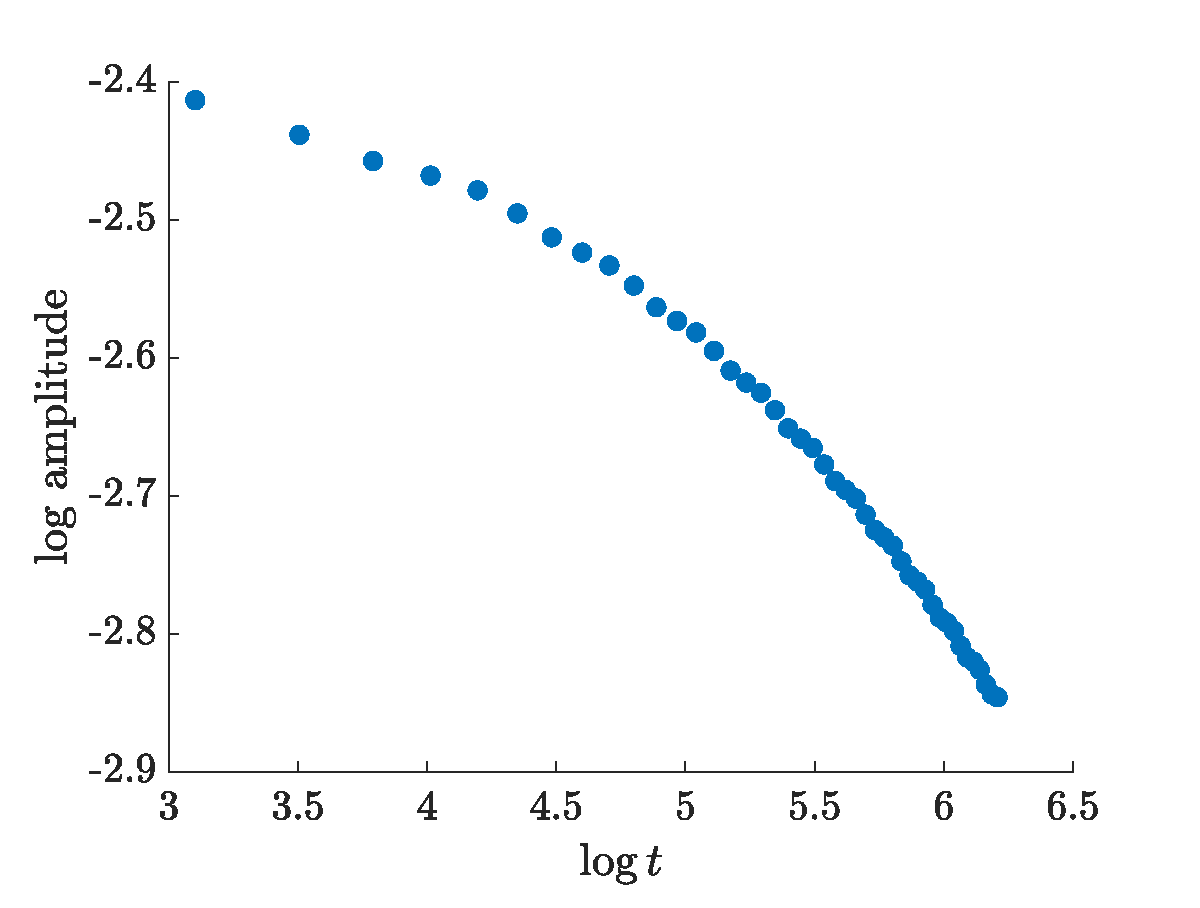
\includegraphics[width=6cm]{kinkoscgoldstonek50N200decay.eps}
	\end{tabular}
	\end{center}
	\caption{Left panel shows difference between perturbed solution and kink for the two central nodes for perturbation of central nodes in same direction by 0.1. Two central nodes are shown in blue solid and red dotted lines. Right panel is log-log plot of amplitude of oscillations vs. $t$ $N=200$ grid points for kink, $d = 0.5$, timestepping using 4th order Runge-Kutta method with step size 0.05. Goldstone mode eigenvalue is $0.57184i$.} 
	\label{fig:kinktimestepresonance}
\end{figure}

For a kink-antikink, the pair of Goldstone mode eigenfunctions suggests that there will be two corresponding normal modes of oscillations for the central nodes of the two kinks: an in-phase mode and an out-of-phase mode. These can be seen in \cref{fig:kaktimestep}. There will similarly be two normal modes corresponding to the pair of edge mode eigenfunctions.

\begin{figure}[H]
	\begin{center}
	\begin{tabular}{cc}
	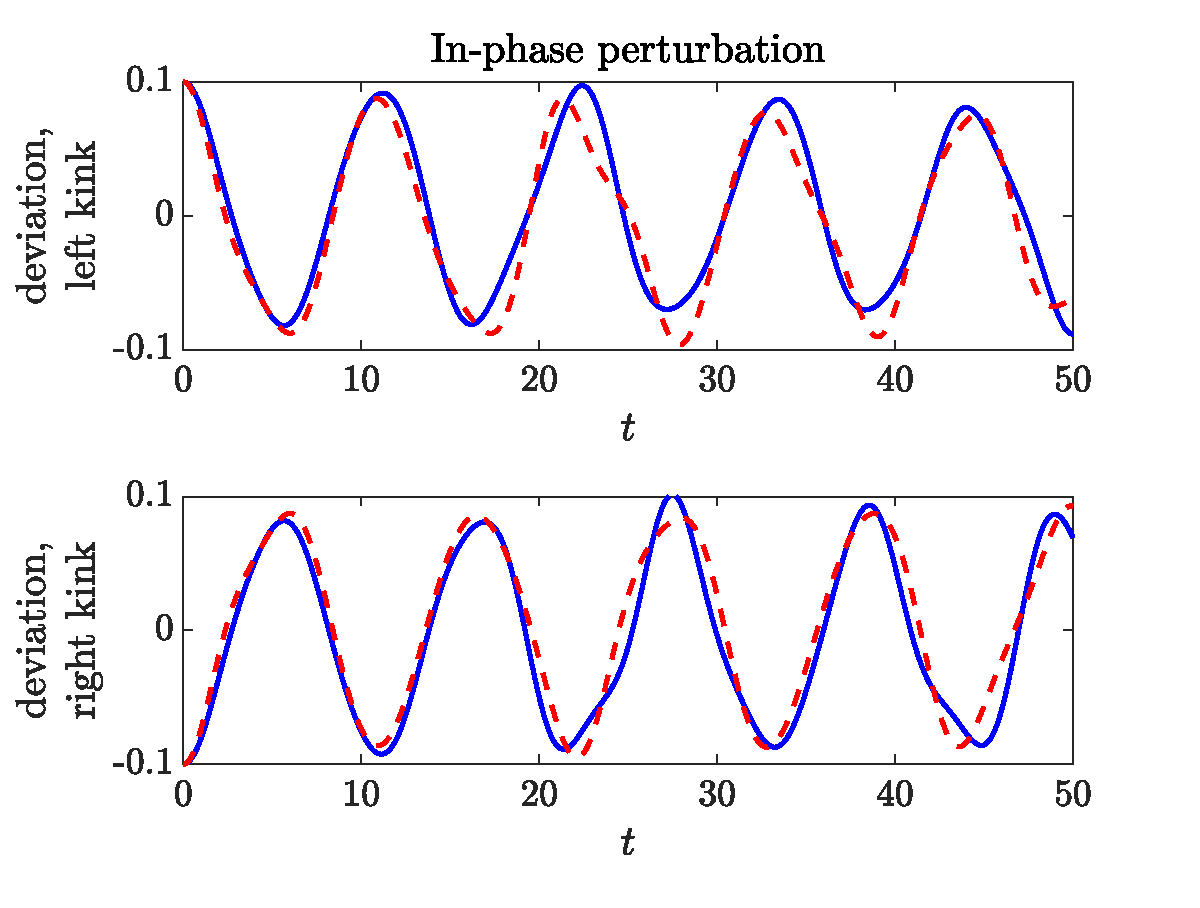
\includegraphics[width=6cm]{kakoscG1.eps} &
	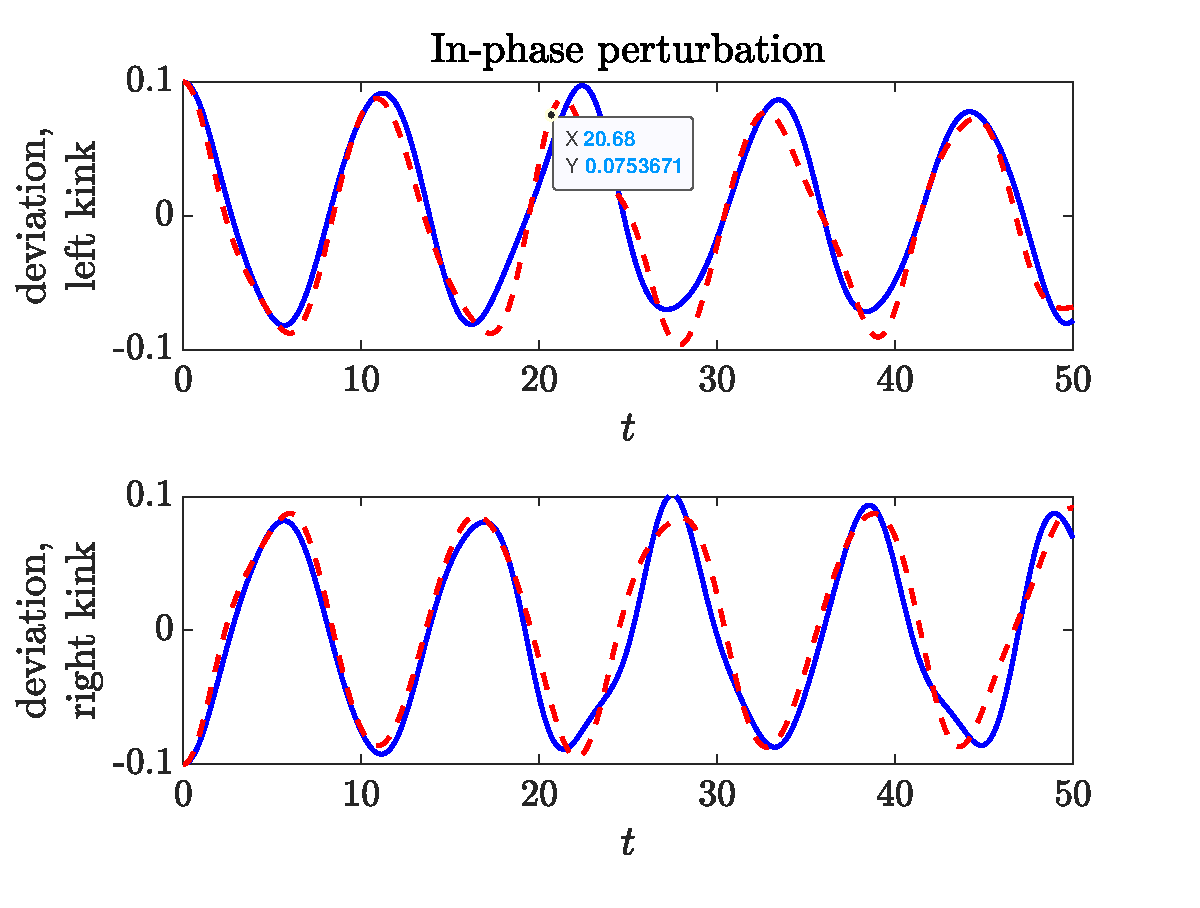
\includegraphics[width=6cm]{kakoscG2.eps} 
	\end{tabular}
	\end{center}
	\caption{Timestepping of perturbation kink-antikink solution. In the left panel, the central nodes of both kinks are perturbed by 0.1 in the same direction. In the right panel, the central nodes of the left kink are perturbed by 0.1, and the central nodes of the right kink are perturbed by -0.1. $d = 0.5$, timestepping using 4th order Runge-Kutta method, step size 0.04.} 
	\label{fig:kaktimestep}
\end{figure}


\section{Proof of \cref{th:KaKexists}}

The proof is an adaptation of the proofs of Theorems 1 and 3 in \cite{Parker2020}. First, we rewrite the system as a fixed point problem. Expanding $F(u)$ in a Taylor series about $c_i K(n)$, we get
\begin{align}\label{eq:Feq0}
F(U_i^\pm(n)) &= F(c_i K(n) + \tilde{U}_i^-(n)) = 
D F(c_i K(n)) \tilde{U}_i^\pm(n) + G(\tilde{U}_i^\pm(n)),
\end{align}
where $G(\tilde{U}_i^\pm(n)) = \mathcal{O}(|\tilde{U}_i^\pm|^2)$ with $G(0) = 0$ and $DG(0) = 0$. Since $f(u)$ is odd, $f'(u)$ is even, thus $D F(c_i K(n)) = D F(K(n))$, and equation \cref{eq:Feq0} becomes
\begin{align}\label{eq:Feq1}
F(U_i^\pm(n)) &= 
D F(K(n)) \tilde{U}_i^\pm(n) + G(\tilde{U}_i^\pm(n).
\end{align}
Since the pieces $U_i^\pm$ in the ansatz \cref{eq:Upiecewise} must match at their endpoints, we obtain the following system of equations for the remainder functions $\tilde{U}_i^\pm$
\begin{align}
\tilde{U}_i^\pm(n+1) &= D F(K(n)) \tilde{U}_i^\pm(n) + G(\tilde{K}_i^\pm(n)) \label{eq:Wsystem1} \\
\tilde{U}_i^+(N_i^+) - \tilde{U}_{i+1}^-(-N_i^-) &= d_i \label{eq:Wsystem2} \\
\tilde{U}_i^+(0) - \tilde{U}_i^-(0) &= 0. \label{eq:Wsystem3}
\end{align}
where
\begin{align}\label{didef}
	d_i &= c_{i+1} K(-N_i^-) - c_i K(N_i^+).
\end{align}
Let $\Phi(m, n)$ be the evolution operators for the linear difference equation 
\[
V(n+1) = D F(K(n)) V(n).
\]
By the stable manifold theorem, $|K(n) - S^+| \leq C r^{-|n|}$ for $n \geq 0$ and $|K(n) - S^-| \leq C r^{-|n|}$ for $n \leq 0$, thus $| DF(K(n)) - DF(S^\pm)| \leq C r^{-|n|}$. Since $S^\pm$ are hyperbolic fixed points, we can decompose the evolution operator $\Phi(m, n)$ in exponential dichotomies on $\Z^\pm$ by \cite{Parker2020}*{Lemma 2}. The proof then follows that of \cite{Parker2020}*{Theorems 1 and 3}. Briefly, we write equation \cref{eq:Wsystem1} in fixed-point form using the discrete variation of constants formula together with projections on the stable and unstable subspaces of the exponential dichotomy. As long as $N$ is sufficiently large, we use the implicit function theorem to solve for the remainder functions $\tilde{U}_i^\pm$ as well as the matching conditions \cref{eq:Wsystem2} and \cref{eq:Wsystem3}. Since $W^u(S^-)$ and $W^s(S^+)$ intersect transversely, we have the decomposition $\R^2 = T_{K(0)}W^u(S^-)\oplus T_{K(0)}W^s(S^+)$, thus as in the proof of \cite{Parker2020}*{Theorem 3}, solving \cref{eq:Wsystem3} does not involve jump conditions. The estimates \cref{eq:Uestimates} follow from the proof \cite{Parker2020}*{Theorem 3} (see in particular Lemma 4).

\section{Proof of \cref{th:stability}}

For the multi-kink solution $U(n)$, we will take an ansatz which is a piecewise perturbation of $V_0(n)$. Let
\begin{equation}\label{eq:Viansatz}
V_i^\pm(n) = d_i c_i V_0(n) + W_i^\pm(n),
\end{equation}
where $d_i \in \C$ and $c_i = (-1)^{i+1}$. Substituting this into \cref{eq:EVPdyneq} and simplifying using \cref{eq:V0eq}, the eigenvalue problem becomes
\begin{equation}\label{eq:Weq1}
\begin{aligned}
W_i^\pm(n+1)
&= DF(K(n)) W_i^\pm(n) + \omega_0 B W_i^\pm(n) \\
&\qquad + [G_i^\pm(n) + (\omega - \omega_0) B](d_i c_i V_0(n) W_i^\pm(n)),
\end{aligned}
\end{equation}
where
\begin{equation}\label{eq:Gipm}
G_i^\pm(n) = DF(U_i^\pm(n)) - DF(K(n)),
\end{equation}
and we used the fact that $DF(c_i K(n)) = DF(K(n))$ from the previous section. Using \cref{eq:Aomegaeq}, we rewrite \cref{eq:Weq1} as
\begin{align}\label{eq:Weq2}
W_i^\pm(n+1)
&= A(n; \omega_0) W_i^\pm(n) + [G_i^\pm(n) + (\omega - \omega_0) B](d_i c_i V_0(n) + W_i^\pm(n)).
\end{align}

In addition to solving \cref{eq:Weq2}, the eigenfunction must satisfy matching conditions at $n = \pm N_i$ and $n = 0$. Thus the system of equations we need to solve is
\begin{equation}\label{eq:eigWsystem1}
\begin{aligned}
& W_i^\pm(n+1)
= A(n; \omega_0) W_i^\pm(n) + [G_i^\pm(n) + (\omega - \omega_0) B](d_i c_i V_0(n) + W_i^\pm(n))\\
& W_i^+(N_i^+) - W_{i+1}^-(-N_i^-) = D_i d \\
& W_i^+(0) - W_i^-(0) = 0,
\end{aligned}
\end{equation}
where
\begin{equation}\label{defDid}
D_i d = d_{i+1} c_{i+1} V_0(-N_i^-) - d_i c_i V_0(N_i^+)
\end{equation}

Let $\Phi(m, n)$ be the evolution operator for the variational equation 
\begin{equation}\label{eq:vareq1}
	V(n+1) = A(n; \omega_0) V(n).
\end{equation}
Since we have the exponential decay \cref{eq:A0decay}, by \cite{Parker2020}*{Lemma 2}, we can decompose the evolution operator $\Phi(m, n)$ in exponential dichotomies on $\Z^\pm$. In particular, we have the estimates 
\begin{equation}\label{eq:dichotomyest}
\begin{aligned}
&|\Phi_+^s(m, n)| \leq C r_0^{m - n} && 0 \leq n \leq m \\
&|\Phi_+^u(m, n)| \leq C r_0^{n - m} && 0 \leq m \leq n \\
&|\Phi_-^s(m, n)| \leq C r_0^{m - n} && n \leq m \leq 0 \\
&|\Phi_-^u(m, n)| \leq C r_0^{n - m} && m \leq n \leq 0 \:,
\end{aligned}
\end{equation}
for the evolution operator on the stable and unstable subspaces of the exponential dichotomy. Furthermore, letting $E^{s/u}$ be the stable and unstable eigenspaces of $A_0$ and $P_0^{s/u}$ the corresponding eigenprojections, we have the decay rates
\begin{equation}\label{eq:eigendecay}
	|P_\pm^{s/u}(n) - P_0^{s/u}| \leq C r^{-|n|},
\end{equation}
where $P_\pm^{s/u}(n) = \Phi_\pm^{s/u}(n, n)$ are the stable and unstable projections for the exponential dichotomy. We note that the decay rates in \cref{eq:dichotomyest} involve the eigenvalues for the matrix $A_0$, whereas those from \cref{eq:eigendecay} come from \cref{eq:A0decay}. 

The variational equation \cref{eq:vareq1} has a bounded solution $V_0(n) = (v_0(n), v_0(n-1))$, and the adjoint variational equation 
\begin{equation}\label{eq:adjvareq1}
	Z(n) = A(n; \omega_0)^* Z(n+1)
\end{equation}
has a bounded solution 
\begin{equation}\label{eq:Z0}
	Z_0(n) = (-v_0(n-1), v_0(n)),
\end{equation}
which is orthogonal to $Z_0(n)$. By the stable manifold theorem,
\begin{equation}\label{eq:VZ0estimates}
	\begin{aligned}
		V_0(n) &\leq C r_0^{-|n|} \\
		Z_0(n) &\leq C r_0^{-|n|}.
	\end{aligned}
\end{equation}

As in \cites{Parker2020,Sandstede1998}, we will not in general be able to solve the system \cref{eq:eigWsystem1}. Instead, since $\R^2 = \spn\{ V_0(0), Z_0(0) \}$, we relax the third equation in \cref{eq:eigWsystem1} to obtain the system of equations
\begin{equation}\label{eq:eigWsystem2}
	\begin{aligned}
	& W_i^\pm(n+1)
	= A(n; \omega_0) W_i^\pm(n) + [G_i^\pm(n) + (\omega - \omega_0) B](d_i c_i V_0(n) + W_i^\pm(n))\\
	& W_i^+(N_i^+) - W_{i+1}^-(-N_i^-) = D_i d \\
	&W_i^+(0) - W_i^-(0) \in \C Z_0(n),
	\end{aligned}
\end{equation}
Using Lin's method, we will be able to find a unique solution to this system, but this solution will generically have $m$ jumps at $n = 0$ in the direction of the adjoint solution $Z_0(0)$. A solution to \cref{eq:eigWsystem2} is therefore an eigenfunction if and only if the $m$ jump conditions
\begin{equation}
	\xi_i = \langle Z_0(0), W_i^+(0) - W_i^-(0) \rangle = 0
\end{equation}
are satisfied. Since $G_i^\pm(n) = \mathcal{O}(\tilde{U}_i^\pm(n))$, we have the same estimates for $G_i^\pm(n)$ as we do for $\tilde{U}_i^\pm$ in \cref{eq:Uestimates}. The terms in \cref{eq:eigWsystem2} are the same as in \cite{Parker2020} with the addition of a term of the form $G_i^\pm(n) V_0(n)$. To estimate that term, we combine the estimates \cref{eq:Uestimates} and \cref{eq:VZ0estimates}. For the interior pieces, we have
\begin{align*}
| G_i^-(n) V_0(n) | &\leq C r^{-N_{i-1}^-} r^{-(N_{i-1}^- + n)} r_0^n \\
&\leq C r^{-2 N_{i-1}^-} \left(\frac{r}{r_0}\right)^{-n} \\
&\leq C \left(\frac{r}{r_0}\right)^{\max\{N_1, \dots, N_m\}} r^{-2 N} \\
&\leq C r^{-2 N} ,
\end{align*}
where in the last step we used the fact that $r_0$ is fixed (it depends only on $\omega_0$), as are the distances $N_i$. The constant will be larger as $r_0$ decreases, which occurs as the eigenvalue $\lambda_0$ gets closer to the continuous spectrum boundary. The estimate for $G_i^+(n) V_0(n)$ is similar, and the estimates for the two exterior pieces are stronger. Thus we have the two uniform estimates
\begin{equation}\label{eq:unifest}
	\begin{aligned}
		\|G_i^\pm\| \leq C r^{-N} \\
		\|G_i^\pm V_0(n) \| \leq C r^{-2 N}.
	\end{aligned}
\end{equation}

The proof then follows as in \cites{Parker2020,Sandstede1998}. First, we write equation \cref{eq:Weq1} as a fixed point problem using the discrete variation of constants formula together with projections on the stable and unstable subspaces of the exponential dichotomy. Let $\delta > 0$ be small, and choose $N$ sufficiently large so that $r^{-N} < \delta$. Define the spaces
\begin{align*}
V_W &= \ell^\infty([-N_{i-1}, 0]) \oplus \ell^\infty([0, N_i])  \\
V_a &= \bigoplus_{i=0}^{n-1} E^u \oplus E^s \\
V_b &= \bigoplus_{i=0}^{n-1} \ran P_-^u(0) \oplus \ran P_+^s(0)\\
V_\lambda &= B_\delta(\omega_0) \subset \C \\
V_d &= \C^d.
\end{align*}
Then for
\begin{align*}
&W = (W_i^-, W_i^+) \in V_W  && a = (a_i^-, a_i^+) \in V_a \\
&\lambda \in V_\lambda  &&b = (b_i^-, b_i^+) \in V_b,
\end{align*}
the fixed point equations for the eigenvalue problem are
\begin{equation*}\label{fpeig}
\begin{aligned}
W_i^-(n) &= 
\Phi_s^-(n, -N_{i-1}^-) a_{i-1}^- + \sum_{j = -N_{i-1}^-}^{n-1} \Phi_s^-(n, j+1)
[G_i^-(j) + (\omega - \omega_0) B](d_i c_i V_0(j) + W_i^-(j))
 \\
&+ \Phi_u^-(n, 0) b_i^- - \sum_{j = n}^{-1} \Phi_u^-(n, j+1) 
[G_i^-(j) + (\omega - \omega_0) B](d_i c_i V_0(j) + W_i^-(j))\\
W_i^+(n) &= \Phi_s^+(n, 0; \theta_i) b_i^+ + \sum_{j = 0}^{n-1} \Phi_s^+(n, j+1) 
[G_i^+(j) + (\omega - \omega_0) B](d_i c_i V_0(j) + W_i^+(j))\\
&+ \Phi_u^+(n, N_i^+) a_i^+ - \sum_{j = n}^{N_i^+-1} \Phi_u^+(n, j+1) 
[G_i^+(j) + (\omega - \omega_0) B](d_i c_i V_0(j) + W_i^+(j)),
\end{aligned}
\end{equation*}
where $a_0^- = a_m^+ = 0$ and the sums are defined to be $0$ if the upper index is smaller than the lower index. We now follow the procedure in the proof of \cite{Parker2020}*{Theorem 2} and invert the system \cref{eq:eigWsystem2} in the following steps. First, we solve for the remainder functions $W_i^\pm(n)$ in the fixed point equations. Then we use the second equation in \cref{eq:eigWsystem2} to solve for the  the initials conditions $a_i^\pm$. Finally, we use the third equation in \cref{eq:eigWsystem2} to solve for the $b_i^\pm$. The procedure is identical to the proof of \cite{Parker2020}*{Theorem 2} with both $\lambda$ and $\lambda^2$ replaced by $\omega - \omega_0$, $\tilde{H}_i^\pm(n)$ replaced by $c_i V_0(n)$, and additional terms of the form $G_i^\pm(n) V_0(n)$, which will be small using the second estimate in \cref{eq:unifest} and will thus be incorporated into the remainder term. Thus we obtain a unique solution to \cref{eq:Wsystem3} generically has $n$ jumps in the direction of $Z_0(0)$ which are given by 
\begin{equation}\label{eq:xieq}
\begin{aligned}
\xi_i &= \langle Z_0(N_i^+), P_0^u D_i d \rangle 
+ \langle Z_0(-N_{i-1}^-), P_0^s D_{i-1} d \rangle - (\omega - \omega_0) d_i c_i M + R(\omega - \omega_0)_i(d),
\end{aligned}
\end{equation}
where $M$ is the Melnikov sum
\[
M = \sum_{j = -\infty}^{\infty} \langle Z_0(j+1), B V_0(j)\rangle,
\]
and the remainder term has uniform bound
\begin{equation}\label{eq:Rbound}
R(\omega - \omega_0)_i(d) \leq
C \left( r^{-N} r_0^{-2N} + |\omega - \omega_0|)(r_0^{-N} + |\omega - \omega_0| )\right).
\end{equation}
For the terms in the Melnikov sum,
\[
\langle Z_0(j+1), B V_0(j)\rangle = \frac{1}{d} \langle (-v_0(j), v_0(j-1))^T, (v_0(j), 0) \rangle
= -\frac{1}{d}v_0(j)^2,
\]
thus it follows that
\begin{equation}\label{eq:M}
M = \sum_{j = -\infty}^{\infty} v_0(j)^2 = \| v_0 \|_{\ell^2},
\end{equation}
which is always positive. It follows from 
\cref{eq:eigendecay} that
\begin{align*}
P_0^u D_i d &= d_{i+1} c_{i+1} V_0(-N_i^-) + \mathcal{O}\left( r^{-N}r_0^{-N}\right) \\
P_0^s D_i d &= -d_i c_i V_0(N_i^+) + \mathcal{O}\left( r^{-N}r_0^{-N}\right).
\end{align*}
Substituting these into \cref{eq:xieq}, we have
\begin{equation*}
\begin{aligned}
\xi_i = \langle Z_0(N_i^+), &V_0(-N_i^-) \rangle d_{i+1} c_{i+1}
- \langle Z_0(-N_{i-1}^-), V_0(N_{i-1}^+) \rangle d_{i-1} c_{i-1} \\
&+ \dfrac{1}{d} (\omega - \omega_0) d_i c_i M+ R(\omega - \omega_0)_i(d),
\end{aligned}
\end{equation*}
where the bound on the remainder term is unchanged. Since $c_i$ and $c_{i+1}$ have opposite signs, this simplifies to 
\begin{align*}
\xi_i = \langle Z_0(N_i^+), V_0(-N_i^-) \rangle d_{i+1}
- \langle Z_0(-N_{i-1}^-), V_0(N_{i-1}^+) \rangle d_{i-1}
- \dfrac{1}{d} (\omega - \omega_0) d_i M
+ R(\omega - \omega_0)_i(d).
\end{align*}
Let
\begin{align*}
a_i &= \langle Z_0(N_i^+), V_0(-N_i^-) \rangle 
= v_0(N_i^+)v_0(-N_i^- - 1) - v_0(N_i^+ - 1)v_0(-N_i^-).
\end{align*}
Using equation \cref{eq:Z0},
\[
\langle Z_0(-N_i^-), V_0(N_i^+) \rangle 
= v_0(N_i^+ - 1)v_0(-N_i^-) - v_0(N_i^+)v_0(-N_i^- - 1) = -a_i,
\]
which we substitute above to obtain
\begin{align}\label{eq:xifinal}
\xi_i = a_i d_{i+1}
+ a_{i-1} d_{i-1}
- \dfrac{1}{d} (\omega - \omega_0) d_i M 
+ R(\omega - \omega_0)_i(d).
\end{align}
The $a_i$ can be simplified further based on symmetries of the eigenfunction $v_0(n)$. For even, intersite eigenfunctions, $v_0(-n) = v_0(n-1)$, thus we have
\begin{align}\label{eq:aievenintersite}
a_i = v_0(N_i^+)v_0(N_i^-) - v_0(N_i^+ - 1)v_0(N_i^- -1).
\end{align}
For odd, intersite eigenfunctions, $v_0(-n) = -v_0(n-1)$, and so
\begin{align}\label{eq:aioddintersite}
	a_i = v_0(N_i^+ - 1)v_0(N_i^- -1) - v_0(N_i^+)v_0(N_i^-).
\end{align}
This can be written as the matrix equation
\begin{equation}\label{eq:matrixAeq}
	\left( A - \frac{1}{d}(\omega - \omega_0)MI + R(\omega-\omega_0)\right)d = 0,
\end{equation}
where $A$ is defined by \cref{eq:matrixA}, which has a nontrivial solution if and only if
\begin{equation}\label{eq:matrixdeteq}
	E(\omega - \omega_0) = 
	\det \left( A - \frac{1}{d}(\omega - \omega_0)MI + R(\omega-\omega_0)\right)d = 0.
\end{equation}
Let $\{ \mu_1, \dots, \mu_{m} \}$ be the eigenvalues of $A$, which are real since $A$ is symmetric. They are also distinct by \cite{Jirari1995}*{Corollary 2.2.7}, since the eigenvalue problem $(A - \mu I) v = 0$ is equivalent to the Sturm-Liouville difference equation with Dirichlet boundary conditions
\begin{equation*}
\begin{aligned}
\nabla( p_j \Delta d_j ) + q_j &= \mu d_j && \qquad j = 1, \dots, m \\
d_0 &= 0 \\
d_{m+1} &= 0,
\end{aligned}
\end{equation*}
where $p_j = a_j$, $q_j = a_j + a_{j-1}$, $\Delta$ is the forward difference operator $(\Delta f)_j = f_{j+1} - f_j$ and $\nabla$ is the backward difference operator $(\nabla f)_j = f_j - f_{j-1}$. 

Following the proof of \cite{Parker2020}*{Theorem 5}, we can use the implicit function theorem to solve for $\omega - \omega_0$ to get the $m$ solutions
\begin{align*}
	\omega_j &= \omega_0 + \frac{d \mu_j}{M} + \mathcal{O}(r_0^{-3N}) && j = 1, \dots, m.
\end{align*}
Since $\mu_j = \mathcal{O}(r_0^{-2N})$, $\omega_0 < 0$, and $\omega$ must be real, $\omega_j < 0$ for sufficiently small $N$. The corresponding eigenvalues are $\lambda_j = \pm \sqrt{\omega_j}$, which are on the imaginary axis.

\bibliographystyle{amsplain}
\bibliography{DKG.bib}

\end{document}